\documentclass[11pt]{article}

\usepackage[margin=1.1in]{geometry}
\usepackage{amsmath,amssymb,amsthm}
\usepackage{mathtools}
\usepackage{booktabs}
\usepackage{tikz}
\usetikzlibrary{arrows.meta,positioning,fit,backgrounds}
\usepackage{xcolor}
\usepackage{enumitem}
\usepackage[colorlinks=true,linkcolor=blue!60!black,citecolor=blue!60!black,urlcolor=blue!60!black]{hyperref}
\usepackage{microtype}
\usepackage{graphicx}

\newtheorem{theorem}{Theorem}[section]
\newtheorem{lemma}[theorem]{Lemma}
\newtheorem{definition}[theorem]{Definition}
\newtheorem{example}[theorem]{Example}
\newtheorem{claim}[theorem]{Claim}
\newtheorem{openq}[theorem]{Open Question}
\newtheorem{proposition}[theorem]{Proposition}
\newtheorem{corollary}[theorem]{Corollary}
\newtheorem{remark}[theorem]{Remark}
\newtheorem{vc}{VC}
\newtheorem*{finding}{Finding}

% Paper-style notation
\newcommand{\vis}{\xrightarrow{\mathsf{vis}}}
\newcommand{\rc}{\xrightarrow{\mathsf{rc}}}
\newcommand{\loC}{\xrightarrow{\mathsf{lo}_{C}}}
\newcommand{\comm}{\rightleftarrows}
\newcommand{\ncomm}{\not\rightleftarrows}
\newcommand{\add}{\mathsf{add}}
\newcommand{\rem}{\mathsf{rem}}
\newcommand{\enb}{\mathsf{enable}}
\newcommand{\dsb}{\mathsf{disable}}
\newcommand{\Merge}{\mathsf{merge}}
\newcommand{\mergeL}{\mathsf{mergeL}}
\newcommand{\Sinit}{\sigma_0}
\newcommand{\loE}[1]{\mathsf{lo}^{#1}}
\newcommand{\dow}[1]{{\downarrow}#1}
\newcommand{\co}{\mathsf{CoreVCs3CD}}
\newcommand{\fd}{\mathsf{FeasibleDeltaVCs3}}
\newcommand{\cd}{\mathsf{CDVC3}}
\newcommand{\lean}[1]{\texttt{#1}}
\newcommand{\M}[1]{\mathcal{#1}}

% Conditioned-part notation (from the end-to-end note)
\newcommand{\st}{\sigma}
\newcommand{\ini}{\st_0}
\newcommand{\dodo}{\mathsf{do}}
\newcommand{\merge}{\mathsf{merge}}
\newcommand{\resolve}{\mathsf{resolve}}
\newcommand{\anc}{\mathsf{anc}}
\newcommand{\contains}{\mathsf{live}}
\newcommand{\recList}{\mathsf{rec}}
\newcommand{\eqobs}{\approx}
\newcommand{\fold}{\mathsf{fold}}
\newcommand{\Inv}{\mathsf{Inv}}
\newcommand{\app}{\mathsf{app}}
\newcommand{\sigmacan}{\st^{\ast}}
\newcommand{\RVF}{\textsf{RecPathFaithful}}
\newcommand{\Faithful}{\textsf{Faithful}}
\newcommand{\ChainFaithful}{\textsf{ChainFaithful}}

\title{\bfseries A Mechanized Metatheory for Mergeable Replicated Data Types:\\
\large RA-linearizability under three-way merge --- eight verification
conditions, a conditioned generalization, and the tombstone-free RGA
end-to-end}
\author{Sal metatheory note\\ \small FP Launchpad, IIT Madras}
\date{July 7, 2026}

\begin{document}
\maketitle

\begin{abstract}
\noindent
Mergeable replicated data types (MRDTs) resolve concurrent divergence by a
\emph{three-way} merge $\mergeL(l,a,b)$: the two divergent states $a,b$
are reconciled relative to their lowest common ancestor $l$ in a git-like
version DAG. The Neem methodology reduces RA-linearizability of an MRDT to
a fixed catalogue of per-data-type verification conditions (VCs), tied
together by a once-and-for-all soundness meta-theorem. Mechanizing that
meta-theorem in Lean~4, we find that its central induction is unsound as
written --- a reachable, fully LCA-legal execution of a legal add-wins
MRDT defeats every bottom-up peel the proof can make --- that the paper's
own LCA lemma, while true, has a gap in its proof, and that no repair can
lean on either of the two obvious crutches: the LCA argument cannot be
forgotten (the counter MRDT provably admits no binary, CRDT-style
collapse), and no lattice-flavoured contract is available (the lattice
laws are equations over free tuples --- the wrong instances for an
LCA-aware merge --- and no usable order survives). What works
is a \emph{delta} discipline: three unconditional relational VCs on
$\mathsf{rc}$, one merge symmetry, three \emph{feasibility-conditioned}
redistribution laws, and a single contextual \emph{causal-delta} equation
--- eight VCs in all --- from which every reachable configuration of the
replicated store is RA-linearizable, \emph{per version}. All of it is
mechanized in Lean~4 with zero \lean{sorry}s, and the VC set is validated
in the strongest currency available: eleven of the twelve production MRDTs
of the Sal repository --- OR-sets, an enable-wins flag, counters, grow-only
set and map, a tombstone RGA, Peritext, the multi-valued register and the
add-wins priority queue --- carry kernel-checked end-to-end
RA-linearizability theorems through it. The one data type
provably \emph{outside} the VC set --- the tombstone-free RGA, whose
commutation holds only on reachable states --- is hosted by a
\emph{conditioned} extension of the metatheory grown from this note's own
open questions: a kernel-checked end-to-end theorem gives
RA-linearizability \emph{up to observational equivalence} at every
reachable configuration, from a single honest-delivery assumption. This
note is the complete, self-contained account: what an MRDT is and how to
describe one (\S\ref{sec:mrdts}), the corrected flat metatheory and its
validation (\S\ref{sec:setting}--\S\ref{sec:catalog}), the conditioned
metatheorem with its pen-and-paper end-to-end proof for the tombstone-free
RGA (\S\ref{sec:condmeta}--\S\ref{sec:actual}), the open questions, and
the mechanization map.
\end{abstract}

\tableofcontents

\section{Introduction}

An MRDT execution looks like a git history: replicas fork, apply
operations locally, and merge. Unlike a state-based CRDT, whose binary
merge must reconcile two states with no memory of their common past, an
MRDT's merge receives a third argument --- the state at the \emph{lowest
common ancestor} (LCA) of the two versions being merged --- and may use it
to compute \emph{deltas}: what each side did since the fork. The
paradigmatic example is the counter,
\[
  \mergeL(l,a,b) \;=\; a + b - l,
\]
which adds the two sides' increments-since-$l$ instead of double-counting
their common past (Figure~\ref{fig:counter}).

\begin{figure}[t]
\centering
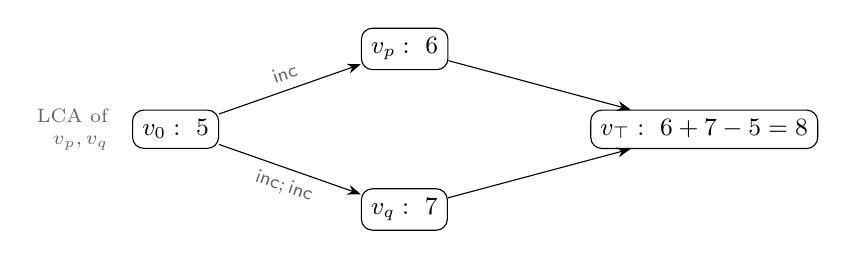
\begin{tikzpicture}[>=Stealth, node distance=0.75cm and 1.5cm,
  ver/.style={draw, rounded corners, inner sep=3.5pt, font=\small},
  lbl/.style={font=\scriptsize, text=black!60}]
\node[ver] (v0) {$v_0:\ 5$};
\node[ver, above right=0.5cm and 1.8cm of v0] (a1) {$v_p:\ 6$};
\node[ver, below right=0.5cm and 1.8cm of v0] (b1) {$v_q:\ 7$};
\node[ver, below right=0.5cm and 1.8cm of a1] (m) {$v_\top:\ 6+7-5 = 8$};
\draw[->] (v0) -- node[lbl, above, sloped]{$\mathsf{inc}$} (a1);
\draw[->] (v0) -- node[lbl, below, sloped]{$\mathsf{inc};\mathsf{inc}$} (b1);
\draw[->] (a1) -- (m);
\draw[->] (b1) -- (m);
\node[lbl, left=0.18cm of v0, align=right] {LCA of\\$v_p,v_q$};
\end{tikzpicture}
\caption{The counter MRDT. Both branches inherit the $5$ from the fork
point; the LCA argument lets the merge count each branch's \emph{delta}
exactly once. No binary merge of $6$ and $7$ alone can recover $8$: the
information ``how much is shared'' lives in the DAG, and the LCA argument
is how the data type reads it.}
\label{fig:counter}
\end{figure}

The Neem methodology (OOPSLA~2025) promises a clean division of labour:
the data-type designer discharges a fixed catalogue of equations over
$\mathsf{do}$, $\mergeL$ and the conflict-resolution relation
$\mathsf{rc}$ --- mostly by SMT --- and a soundness meta-theorem, proved
once, converts those VCs into \emph{RA-linearizability} of every reachable
configuration. This note documents what a Lean~4 mechanization of that
meta-theorem, in the full \textbf{ternary, version-DAG} setting, found:
the meta-theorem's central induction is unsound as written, and for
LCA-sensitive data types several of the catalogue's merge VCs are false
in principle when quantified over all states. It also develops the
corrected metatheory: a set-relative linearization order, canonical
states $\sigma(E)$ (each event set determines a unique state), and a
ternary \emph{Join Lemma} whose induction
consumes a small, contextual VC surface. Its contributions:

\begin{enumerate}[leftmargin=2em]
\item \textbf{The paper's LCA lemma is true but its proof has a gap}
  (\S\ref{sec:lca}): $L(v_\ell) = L(v_1) \cap L(v_2)$ holds, but only as a
  \emph{reachability invariant} of the store, whose proof needs a
  generator-uniqueness induction the paper silently assumes. We mechanize
  the transition system and the invariant.
\item \textbf{The soundness proof has a fully LCA-legal defeater}
  (\S\ref{sec:defeater}): a reachable configuration of a legal add-wins
  MRDT --- its final merge sitting at an honest LCA --- on which every
  bottom-up peel of the paper's derivation rules is stuck. The
  meta-theorem must be rebuilt, not patched.
\item \textbf{The lattice contract does not transfer; a delta contract does}
  (\S\ref{sec:whydelta}): the lattice laws are equations over \emph{free}
  tuples --- the wrong instances for an LCA-aware merge. Side-idempotence
  $\mergeL(l,a,a) = a$ with $l$ free fails for the counter ($2a-l$), but
  its only DAG-honest instance has $l = a$ (the LCA of a version with
  itself \emph{is} that version), where it holds trivially; and when two
  \emph{distinct} histories reach equal side states, $2a-l$ is the
  \emph{correct} merge --- both branches' increments count --- not an
  idempotence failure. The induced orders degenerate, and the honest
  associativity law has \emph{four distinct LCAs} and holds only on
  feasible tuples. The moral: the algebra of an LCA-aware merge is an
  algebra of \emph{causal histories}, not of concrete states. What
  replaces the lattice laws is a two-law \emph{delta contract} --- redistribution identities in which the LCA
  slot does, by arithmetic, the job idempotence does order-theoretically
  for CRDTs.
\item \textbf{Eight VCs suffice} (\S\ref{sec:vcs}--\S\ref{sec:adequacy}):
  three relational VCs on $\mathsf{rc}$ (one of them carrying a
  different-replica guard --- same-replica pairs are ordered by program
  order, and demanding $\mathsf{rc}$ cover them is unsatisfiable for
  real data types), merge symmetry, three
  feasibility-conditioned delta laws, and one contextual \emph{causal-delta}
  equation. The adequacy theorem is per \emph{version}: every version in
  the store, LCAs included, linearizes.
\item \textbf{The VC set is validated on the production catalogue}
  (\S\ref{sec:catalog}): eleven of the twelve MRDTs shipped in Sal ---
  OR-set, an optimized OR-set, enable-wins flag, grow-only set and map,
  increment-only and PN counters, a tombstone RGA, Peritext, the
  multi-valued register and the add-wins priority queue --- are
  discharged end-to-end, kernel-checked; the twelfth, the tombstone-free
  RGA, goes through the conditioned framework. The sweep produces an empirical
  \emph{class map} of which data types need which strength of contract,
  with two surprises: tombstones are a metatheoretic trivializer, and
  commutativity class and delta class are independent axes.
\item \textbf{The eight VCs are one instance of a closure-indexed
  contract} (\S\ref{sec:open}): a mechanized investigation of the note's
  own open questions establishes that the ``second route'' asymmetry
  (\S\ref{sec:adequacy}) is not a defect to be reunified but a
  \emph{closure parameter} the data type declares; a single soundness
  bridge covers both strengths, and \emph{all nine} production discharges
  route through it unchanged. The same investigation refutes the obvious
  attacks on the two remaining frontiers --- it defeats even the commuting
  \textsc{2-OP} rule on the defeater, pins the feasible-update-layer
  feasibility notion, and characterizes exactly why the tombstone-free RGA
  resists (it converges, but through semantic commutation the pointwise
  bubble cannot see). Pushed to its end, the investigation \emph{hosts}
  the tombstone-free RGA: the swap architecture itself is refuted at merge
  unions, and a conditioned metatheory --- an observational quotient, a
  canonical-witness discipline per version, and a generation discipline
  derived from born accuracy --- proves it RA-linearizable up to
  observational equivalence, end-to-end under honest delivery. All
  kernel-checked.
\end{enumerate}

Everything stated as a theorem below is mechanized with zero
\lean{sorry}s; \S\ref{sec:mech} maps statements to Lean names and files
(foundations under \lean{Framework/}, metatheorems under
\lean{Metatheory/}, negative results under \lean{Refutations/}, the
per-RDT instances under \lean{MRDT\_Instances/}, the investigation record
under \lean{Development/}; each cited theorem kernel-checked).


\section{Mergeable replicated data types, by definition and example}
\label{sec:mrdts}

\paragraph{Data type and implementation.} A replicated data type of
\emph{type} $\tau = \langle O_\tau, Q_\tau, \mathit{Val}_\tau\rangle$
exposes a set of update operations $O_\tau$, a set of query operations
$Q_\tau$, and a domain of query return values $\mathit{Val}_\tau$. An
\emph{MRDT implementation} of $\tau$ is a tuple
\[
  \M{D} \;=\; \langle \Sigma,\; \Sinit,\; \mathsf{do},\; \mergeL,\;
  \mathsf{query},\; \mathsf{rc} \rangle ,
\]
where $\Sigma$ is the space of replica states with initial state
$\Sinit$; $\mathsf{do} : \Sigma \times \M{E} \to \Sigma$ applies an
\emph{event} --- an update-operation instance $e = (t, r, o)$ carrying a
globally unique timestamp $t$, its origin replica $r$, and the operation
$o \in O_\tau$; $\mergeL : \Sigma^3 \to \Sigma$ is the three-way merge,
whose first argument is the state at the lowest common ancestor of the
two versions being merged; $\mathsf{query} : \Sigma \times Q_\tau \to
\mathit{Val}_\tau$ reads a state; and $\mathsf{rc} \subseteq O_\tau
\times O_\tau$ is the \emph{conflict-resolution} relation, consulted to
order concurrent non-commuting operations (it is the data-type designer's
declaration of who wins a race). Queries never change state and play no
role in the metatheory; the theory below reads the implementation as
$\langle \Sigma, \Sinit, \mathsf{do}, \mergeL, \mathsf{rc}\rangle$.

\paragraph{Describing an MRDT: the counter.} To describe an MRDT one
gives the five components and, when operations can race, says who wins.
The increment-only counter of Figure~\ref{fig:counter} is the smallest
complete example:
\[
  \Sigma = \mathbb{Z}, \qquad \Sinit = 0, \qquad
  \mathsf{do}(\sigma, (t,r,\mathsf{inc})) = \sigma + 1, \qquad
  \mergeL(l,a,b) = a + b - l, \qquad \mathsf{rc} = \emptyset .
\]
All operations commute, so $\mathsf{rc}$ is empty --- yet the merge
genuinely uses its LCA argument: $a + b$ alone would double-count the
history shared by the two branches, and the $-\,l$ subtracts it exactly
once. This ``read the shared past off the LCA'' pattern recurs
throughout the catalogue.

\paragraph{A data type with races: the OR-set.} The add-wins observed-remove
set stores tagged elements: $\add$ inserts a tag unique to the adding
event, $\rem$ deletes exactly the tags it has \emph{seen}. Sequentially,
a remove after an add deletes it; concurrently the designer declares the
add the winner: $\rem \rc \add$. The merge keeps a tag iff both sides
have it (nobody deleted it) or some side added it since the fork:
\[
  \mergeL(l,a,b) \;=\; (a \cap b) \cup (a \setminus l) \cup (b \setminus l).
\]
The LCA here plays the role a tombstone set plays for the CRDT OR-set:
deletion is absence \emph{relative to} $l$, and the state needs no
graveyard.

\paragraph{The generalized signature.} Both examples' operations make
sense on \emph{every} state: any state can be incremented, any tag can be
added. Such data types are \emph{flat}, and for them the metatheory of
\S\ref{sec:setting}--\S\ref{sec:catalog} quantifies its VCs over all
states. But a data type whose operations carry \emph{preconditions} ---
insert under a node that must exist, delete a node that must be live ---
breaks that quantification: its commutation equations are simply false at
nonsense states. The full signature therefore extends the tuple with
three declarations (\lean{ConditionedMRDTSig}; formalized in
\S\ref{sec:cvcs}):
\[
  \M{D} \;=\; \langle \Sigma, \Sinit, \mathsf{do}, \mergeL, \mathsf{rc},\;
  \Inv,\; \app \rangle
  \quad\text{together with}\quad {\eqobs} \subseteq \Sigma \times \Sigma ,
\]
where $\Inv$ is a state invariant (a shape over-approximation of
reachability), $\app$ an applicability predicate (when an event is
sensible at a state), and $\eqobs$ an observational equivalence (what
queries can distinguish; representation residue is quotiented away).
Commutation is then required only at $\Inv$-states where both events are
applicable. Flat data types take $\Inv = \app = \top$ and
${\eqobs} = {=}$, collapsing the general signature to the plain one ---
one framework, of which \S\ref{sec:setting}--\S\ref{sec:catalog} is the
flat instance and \S\ref{sec:condmeta} onwards the general case.

\paragraph{The running hard example: the tombstone-free RGA.} The
Replicated Growable Array is the list CRDT/MRDT underlying collaborative
text editing: characters are nodes identified by timestamps, each
inserted \emph{after} an anchor node. Production RGAs keep deleted nodes
as \emph{tombstones} because later concurrent inserts may still anchor on
them. The \emph{tombstone-free} RGA deletes physically, and it is
describable in the general signature:
\begin{itemize}[leftmargin=2em,nosep]
\item $\Sigma$: finite forests --- partial maps from node ids to
  (element, anchor id), the root id $0$ never stored; $\Sinit$ the empty
  forest.
\item Operations: $\mathsf{Ins}(e, p, a)$ inserts a fresh node with
  element $e$ under anchor $a$, and $\mathsf{Del}(p, x)$ deletes node
  $x$; both carry a \emph{recorded path} $p$ --- the anchor's (resp.\
  target's) ancestor chain as the issuing replica saw it. $\mathsf{do}$
  resolves the first live entry of $a :: p$ and attaches there; a delete
  removes $x$ physically and \emph{rehomes} $x$'s children to $x$'s
  nearest live ancestor.
\item $\mergeL(l,a,b)$: OR-set survivorship on node ids (present in both
  sides, or born since the fork on one), each survivor re-anchored by
  climbing its recorded chain to the nearest survivor.
\item $\mathsf{rc}$: empty in the directional sense (\lean{Either}) ---
  every pair commutes, but only \emph{conditionally}.
\item $\Inv$: well-formed forest (every stored anchor live or root),
  id-monotone anchors ($\anc(x) < x$), root unstored.
\item $\app$: \emph{accurate} (the recorded path is the target's true
  live ancestor chain in the current state) and \emph{fresh} (the id is
  unused) --- the predicate that holds at an op's generation but not at
  arbitrary replay states, which is where conditioning bites.
\item $\eqobs$: equal live forests --- same nodes, elements and anchors.
\end{itemize}
A three-node example (Figure~\ref{fig:rga-example}) shows why every
piece is needed. Start from the chain $0 \leftarrow 1 \leftarrow 2$ (node $1$ under the root, node $2$
under $1$). $\mathsf{Del}([0], 1)$ removes node $1$ and rehomes $2$ to
the root. A \emph{concurrent} event $(3, r, \mathsf{Ins}(e, [0], 1))$ ---
generated before the delete was seen, anchored on $1$, whose recorded
chain $1 :: [0]$ is $1$'s live ancestor chain at generation --- arrives
after it: the anchor is gone, and the recorded chain is exactly what lets
$\mathsf{do}$ resolve the insert to $1$'s parent $0$, where the delete
rehomed $1$'s children. Commutation of this pair over
\emph{all} states is false (the recorded path can lie about a nonsense
state); at reachable, accurate states it holds. This data type is the
reason the general signature exists, and
\S\ref{sec:condmeta}--\S\ref{sec:actual} prove it RA-linearizable up to
$\eqobs$, end-to-end.

\begin{figure}[t]
\centering
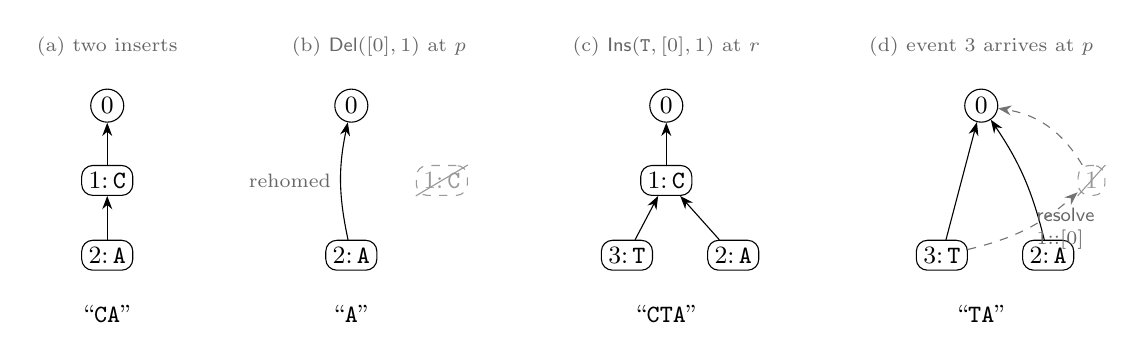
\begin{tikzpicture}[>=Stealth,
  nd/.style={draw, rounded corners, inner sep=2.5pt, font=\small},
  ghost/.style={draw, dashed, rounded corners, inner sep=2.5pt,
    font=\small, text=black!40, draw=black!40},
  rt/.style={draw, circle, inner sep=1.6pt, font=\small},
  lbl/.style={font=\scriptsize, text=black!60},
  doc/.style={font=\small}]
% (a) two inserts
\begin{scope}
\node[lbl] (ta) at (0,0.75) {(a) two inserts};
\node[rt] (a0) at (0,0) {$0$};
\node[nd] (a1) at (0,-0.95) {$1{:}\,\texttt{C}$};
\node[nd] (a2) at (0,-1.9) {$2{:}\,\texttt{A}$};
\draw[->] (a1) -- (a0);
\draw[->] (a2) -- (a1);
\node[doc] at (0,-2.65) {``\texttt{CA}''};
\end{scope}
% (b) physical delete + rehome
\begin{scope}[xshift=3.1cm]
\node[lbl] at (0.35,0.75) {(b) $\mathsf{Del}([0],1)$ at $p$};
\node[rt] (b0) at (0,0) {$0$};
\node[ghost] (b1) at (1.15,-0.95) {$1{:}\,\texttt{C}$};
\draw[black!40] (b1.south west) -- (b1.north east);
\node[nd] (b2) at (0,-1.9) {$2{:}\,\texttt{A}$};
\draw[->] (b2) to[bend left=12] node[lbl, left]{rehomed} (b0);
\node[doc] at (0,-2.65) {``\texttt{A}''};
\end{scope}
% (c) concurrent insert at r, generated against (a)
\begin{scope}[xshift=6.6cm]
\node[lbl] at (0.5,0.75) {(c) $\mathsf{Ins}(\texttt{T},[0],1)$ at $r$};
\node[rt] (c0) at (0.5,0) {$0$};
\node[nd] (c1) at (0.5,-0.95) {$1{:}\,\texttt{C}$};
\node[nd] (c3) at (0,-1.9) {$3{:}\,\texttt{T}$};
\node[nd] (c2) at (1.35,-1.9) {$2{:}\,\texttt{A}$};
\draw[->] (c1) -- (c0);
\draw[->] (c3) -- (c1);
\draw[->] (c2) -- (c1);
\node[doc] at (0.5,-2.65) {``\texttt{CTA}''};
\end{scope}
% (d) delivery after the delete
\begin{scope}[xshift=10.6cm]
\node[lbl] at (0.5,0.75) {(d) event $3$ arrives at $p$};
\node[rt] (d0) at (0.5,0) {$0$};
\node[ghost] (d1) at (1.9,-0.95) {$1$};
\draw[black!40] (d1.south west) -- (d1.north east);
\node[nd] (d3) at (0,-1.9) {$3{:}\,\texttt{T}$};
\node[nd] (d2) at (1.35,-1.9) {$2{:}\,\texttt{A}$};
\draw[->] (d3) -- (d0);
\draw[->] (d2) to[bend right=10] (d0);
\draw[->, dashed, black!55] (d3) to[bend right=14]
  node[lbl, right, align=left]{$\resolve$\\ $1{::}[0]$} (d1);
\draw[->, dashed, black!55] (d1) to[bend right=25] (d0);
\node[doc] at (0.5,-2.65) {``\texttt{TA}''};
\end{scope}
\end{tikzpicture}
\caption{The running example as trees and the text they represent.
Boxes are nodes $\mathit{id}{:}\,\mathit{element}$; arrows point to the
anchor ($\anc$); the document is the depth-first traversal visiting
siblings newest-id first. (a)~Two inserts build the chain
$0 \leftarrow 1 \leftarrow 2$: text ``\texttt{CA}''. (b)~Replica $p$
deletes node $1$ \emph{physically} --- no tombstone remains --- and its
child $2$ is rehomed to $1$'s nearest live ancestor, the root.
(c)~Concurrently, replica $r$ --- which has not seen the delete ---
inserts \texttt{T} after \texttt{C}: event $(3, r,
\mathsf{Ins}(\texttt{T}, [0], 1))$, whose recorded path $1{::}[0]$ is
$1$'s live ancestor chain at generation; at $r$ the text reads
``\texttt{CTA}''. (d)~When event $3$ arrives at $p$ the anchor is gone;
$\resolve$ climbs the recorded path past the dead $1$ to $0$ and
attaches there. Folding the two concurrent events in either order yields
this same forest (``\texttt{TA}'') --- the pair commutes at accurate
states, which is exactly what the recorded path buys and what no static
$\mathsf{rc}$ policy could provide.}
\label{fig:rga-example}
\end{figure}

\section{The ternary setting}
\label{sec:setting}

This section fixes the model: the data-type signature, the replicated
store and its transitions, and the specification the metatheorem must
deliver. The definitions are the paper's, with one correction flagged
where it occurs.

\paragraph{Signature.} An MRDT is $\langle \Sigma, \Sinit, \mathsf{do},
\mergeL, \mathsf{rc}\rangle$ as in \S\ref{sec:mrdts}, read flat for now
($\Inv = \app = \top$, ${\eqobs} = {=}$; the general case resumes in
\S\ref{sec:condmeta}). We write $e(\sigma)$ for
$\mathsf{do}(\sigma,e)$, and $e_1 \comm e_2$ when
$e_1(e_2(\sigma)) = e_2(e_1(\sigma))$ for every $\sigma$.

\paragraph{Executions.} A configuration carries a \emph{store}: a DAG of
versions, each holding a state and the set of events that produced it,
with per-replica heads. Transitions fork a replica, apply a fresh event at
a head, query, or \textbf{merge}: pick heads $v_1, v_2$, find their LCA
$v_\ell$ in the DAG, and install a new version with state
$\mergeL(\sigma_{v_\ell}, \sigma_{v_1}, \sigma_{v_2})$ and event set
$L(v_1) \cup L(v_2)$. Visibility $\vis$ records what each event's issuing
replica had seen.

\paragraph{RA-linearizability, per version.} Write $e_1 \parallel e_2$
when neither $e_1 \vis e_2$ nor $e_2 \vis e_1$ (concurrency).

\begin{definition}[linearization order, set-relative]
\label{def:lo}
For an event set $E$, the order $\loE{E}$ puts $e_1$ before $e_2$ iff
\[
\bigl(e_1 \vis e_2 \;\wedge\; e_1 \ncomm e_2\bigr)
\;\;\vee\;\;
\bigl(e_1 \parallel e_2 \;\wedge\; e_1 \rc e_2 \;\wedge\;
  \neg\,\exists e_3 \in E.\;\; e_2 \vis e_3 \,\wedge\, e_2 \ncomm e_3\bigr):
\]
a visible non-commuting pair is ordered by visibility; a concurrent pair
whose conflict $\mathsf{rc}$ resolves is ordered by $\mathsf{rc}$ ---
unless $e_2$ is already \emph{absorbed} (overwritten) by a later
non-commuting event of $E$. The paper's order $\mathsf{lo}$ is the
variant whose absorber clause ranges over the whole configuration; since
a $\mathsf{lo}$-edge asserts \emph{no absorber anywhere},
$\mathsf{lo} \subseteq \loE{E}$ pointwise, for every $E$.
\end{definition}

\begin{definition}[RA-linearizability]
\label{def:ralin}
A list $\pi = e^1 e^2 \cdots e^n$ \emph{witnesses} a version holding
state $s$ and event set $E$ when (i)~$\pi$ enumerates $E$ without
repetition; (ii)~$\pi$ \emph{extends} $\mathsf{lo}$: $i < j$ implies
$\neg(e^j \mathrel{\mathsf{lo}} e^i)$; and (iii)~$\pi$ \emph{folds} to
the state: $e^n(\cdots e^2(e^1(\Sinit))\cdots) = s$. A configuration is
\emph{RA-linearizable} when \emph{every version in the store} --- not
only the replica heads; LCAs are historical versions and the merge reads
them --- admits a witness. In the general signature the fold clause
(iii) is read up to the data type's observational equivalence,
$e^n(\cdots e^1(\Sinit)\cdots) \eqobs s$ --- the same definition with
its equality parameter generalized; flat data types instantiate
${\eqobs} = {=}$ and this section's form is exactly that instance.
\hfill\lean{IsRALinearizable3}, \lean{IsRALinearizable3Eq}
\end{definition}

Why a set-relative order? One definitional correction is forced at the
outset: for every internal use, the absorber clause must range over the
event set of \emph{the version being linearized}, not over the whole
configuration --- an event can gain absorbers from another branch,
silently cancelling an order edge inside a version whose own state
depends on it (the defeater of \S\ref{sec:defeater} realizes exactly
this). We therefore construct witnesses respecting $\loE{E}$ throughout;
since $\mathsf{lo} \subseteq \loE{E}$, every such witness also extends
the paper's order, and Definition~\ref{def:ralin} is delivered exactly
as the paper states it.

\paragraph{Running examples.} Three data types exercise every corner of
the theory:
\begin{itemize}[leftmargin=2em]
\item the \textbf{counter}: $\Sigma = \mathbb{Z}$,
  $\mathsf{inc}(\sigma) = \sigma+1$, $\mergeL(l,a,b) = a+b-l$; all
  operations commute, but the merge genuinely uses its LCA;
\item the \textbf{OR-set} (tagged add-wins set): elements are tagged by
  the adding event's timestamp; $\rem$ deletes the tags it has seen;
  concurrently, $\rem \rc \add$ resolves in favour of the add. The merge
  keeps an element iff \emph{both} sides have it or \emph{some} side added
  it since the fork:
  \[
    \mergeL(l,a,b) \;=\; (a \cap b) \,\cup\, (a \setminus l) \,\cup\, (b
    \setminus l)
  \]
  --- pointwise, ``if the tag is in $l$, require it in both branches
  (nobody deleted it); otherwise one branch suffices (somebody added
  it).'' Here the LCA acts as a \emph{tombstone set}: deletion is
  represented by \emph{absence relative to} $l$, so the state itself needs
  no graveyard;
\item the \textbf{enable-wins flag}: per-replica pairs
  $(\text{counter},\text{flag})$; enabling bumps your own counter and sets
  your flag; disabling clears all flags; the merge compares each
  replica's counter against the LCA's to decide whether an enable
  ``happened since the fork'' on that replica. Its merge \emph{compares}
  counters rather than accumulating sets --- and that difference will be
  visible in the metatheory (\S\ref{sec:catalog}).
\end{itemize}

\section{Three facts the metatheory must respect}

Before building anything, we record two boundary facts about the
paper's development: its store-level LCA lemma is true but under-proved,
and its soundness induction is refuted by a fully legal execution.
Together they fix the shape of the corrected metatheory --- resting on a
mechanized store invariant (\S\ref{sec:lca}) and built around the join
rather than the sides (\S\ref{sec:defeater}).

\subsection{The LCA lemma is a reachability invariant --- with a gap in the
published proof}
\label{sec:lca}

Everything above silently used:

\begin{lemma}[LCA lemma]
\label{lem:lca}
In every reachable configuration, if $v_\ell$ is an LCA of versions $v_1,
v_2$ in the store's DAG, then $L(v_\ell) = L(v_1) \cap L(v_2)$.
\end{lemma}

This is what lets merge VCs be stated over \emph{event sets}: the state
the merge receives as $l$ is the canonical state of exactly the
intersection of the two sides' histories. The lemma is true --- but it is
a \emph{global induction over the reachable store}, not a local fact. Its
mechanized proof threads a store invariant (all parents allocated; event
sets monotone along edges; and an \emph{origin} invariant --- each event
appears first at a unique generator version) through every transition; the
published proof asserts the generator-uniqueness step without the
induction that sustains it. An erratum-sized gap: the statement survives,
the proof as written does not. (A related boundary fact:
\emph{criss-cross} merges can defeat the \emph{existence} of an
LCA --- they gate merge-enabledness, not the lemma. Open
Question~\ref{oq:crisscross} takes up the extension.)

\subsection{A fully LCA-legal execution defeats the soundness proof}
\label{sec:defeater}

The generic half of the paper's contract is a \emph{bottom-up
linearization} theorem: given linearization witnesses for the two sides
of a merge, construct one for the merged version by repeatedly
\emph{peeling} a final event through $\mergeL$ using the catalogue's
interchange VCs. One might hope the version DAG's discipline --- every
merge sitting at an honest LCA --- keeps the peel supplied with peelable
events. It does not: one staging replica suffices to realize the
intersection of two histories as an honest version, and the merge
induction is stuck.

\begin{example}[the defeater]
\label{ex:defeater}
The data type is a one-key add-wins skeleton with tagged adds:
$\sigma = (A, D) \in 2^{\mathbb{T}} \times 2^{\mathbb{T}}$ with live set
$A \setminus D$; $\add_t$ inserts its tag into $A$; $\rem$ kills
everything it currently sees ($D \coloneqq A \cup D$ --- the
state-dependence is what makes $\add \ncomm \rem$); concurrently
$\rem \rc \add$ (add wins); the merge is componentwise union, ignoring
its LCA argument. A legal MRDT.
Replica $p$ adds ($A_p$), replica $q$ adds ($A_q$). A staging replica $s$
merges both one-add versions, creating $v_s$ with
$L(v_s) = \{A_p, A_q\}$. Now $p$ removes ($R_p$, seeing only $A_p$) and
then merges with $v_s$; symmetrically $q$ removes ($R_q$) and merges with
$v_s$. Figure~\ref{fig:defeater} shows the DAG. The final merge of the two
heads finds $\mathrm{LCA} = v_s$, and
$L(v_s) = \{A_p,A_q\} = L(\text{head}_p) \cap L(\text{head}_q)$ --- the
configuration is fully legal. Now count last events. $p$'s head lives on
exactly $A_q$'s tag, so a state-correct witness must run $R_p$ before
$A_q$, and neither $R_p$ nor $A_p$ can come last: every linearization of
$p$'s head ends in $A_q$. Symmetrically, every linearization of $q$'s
head ends in $A_p$. Yet in the \emph{merged} version every tag is dead,
so its linearizations must end in one of the removes.
The events the induction must peel are \emph{buried} in the very sides
that own them; no ordering of the paper's bottom-up rules applies.
\end{example}

The two removes commute ($\rem \ncomm \add$ but $\rem \comm \rem$), which
invites a particular rescue attempt: the paper's \textsc{BottomUp-2-OP}
rule (\lean{inter\_lca\_2op}) admits the commuting case and could, one
hopes, peel a remove last. It cannot, for a reason that is a one-line
state fact. To peel $o$ last from a side, that side's state must be an
$o$-image --- of the form $\mathsf{do}(\sigma', o)$ with $o$ outermost.
But in the add-wins skeleton \emph{every} $\rem$-output has empty live set
($\rem(A,D) = (A, A\cup D)$), whereas both heads carry a live tag
($\mathrm{head}_p$ lives on $A_q$, $\mathrm{head}_q$ on $A_p$ --- the
opposite add, merged in \emph{after} the local remove). So neither head
is a $\rem$-image, and no bottom-up rule can extract a remove from it. The
tempting linearization $[A_p, R_p, A_q, R_q]$ is a valid witness of the
\emph{merged} version, but its restriction to $\mathrm{head}_q$ folds to
the all-dead state, not $\mathrm{head}_q$'s actual state (live $A_p$): it
is not assembled from a state-correct side witness, which is exactly what
the induction requires. All three facts are mechanized
(\lean{InterLca2op\_Defeater\_Arbiter}: \lean{awset\_rem\_output\_empty},
\lean{no\_inter\_lca\_2op\_rem\_peel\_of\_defeater}, \lean{crack1\_witness}).

\begin{figure}[t]
\centering
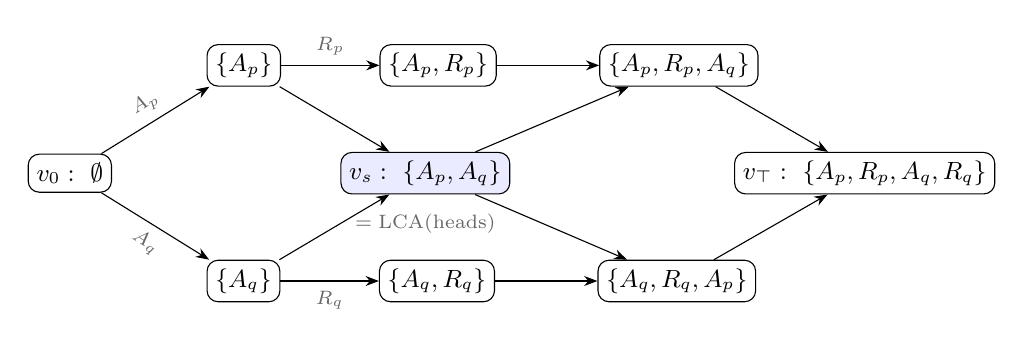
\begin{tikzpicture}[>=Stealth, node distance=0.55cm and 1.35cm,
  ver/.style={draw, rounded corners, inner sep=3pt, font=\small},
  lca/.style={draw, rounded corners, inner sep=3pt, font=\small,
    fill=blue!8},
  lbl/.style={font=\scriptsize, text=black!60}]
\node[ver] (v0) {$v_0:\ \emptyset$};
\node[ver, above right=0.85cm and 1.2cm of v0] (p1) {$\{A_p\}$};
\node[ver, below right=0.85cm and 1.2cm of v0] (q1) {$\{A_q\}$};
\node[lca, right=2.9cm of v0] (s) {$v_s:\ \{A_p,A_q\}$};
\node[ver, right=1.25cm of p1] (p2) {$\{A_p,R_p\}$};
\node[ver, right=1.25cm of q1] (q2) {$\{A_q,R_q\}$};
\node[ver, right=1.3cm of p2] (p3) {$\{A_p,R_p,A_q\}$};
\node[ver, right=1.3cm of q2] (q3) {$\{A_q,R_q,A_p\}$};
\node[ver, right=7.9cm of v0] (top) {$v_\top:\ \{A_p,R_p,A_q,R_q\}$};
\draw[->] (v0) -- node[lbl, above, sloped]{$A_p$} (p1);
\draw[->] (v0) -- node[lbl, below, sloped]{$A_q$} (q1);
\draw[->] (p1) -- (s);
\draw[->] (q1) -- (s);
\draw[->] (p1) -- node[lbl, above]{$R_p$} (p2);
\draw[->] (q1) -- node[lbl, below]{$R_q$} (q2);
\draw[->] (p2) -- (p3);
\draw[->] (s) -- (p3);
\draw[->] (q2) -- (q3);
\draw[->] (s) -- (q3);
\draw[->] (p3) -- (top);
\draw[->] (q3) -- (top);
\node[lbl, below=0.12cm of s] {$=\mathrm{LCA}(\text{heads})$};
\end{tikzpicture}
\caption{The defeater (Example~\ref{ex:defeater}). Nodes are
versions labelled by their event sets; the shaded version $v_s$, created
by a staging replica, realizes $L(\text{head}_p)\cap L(\text{head}_q)$ as
an honest store version, so the final merge is LCA-legal. The removes
$R_p, R_q$ --- the only events a bottom-up derivation may peel last ---
are buried mid-history on their own sides.}
\label{fig:defeater}
\end{figure}

The consequence for the design: the metatheorem cannot be patched
peel-by-peel --- it must be rebuilt on canonical states and a Join Lemma,
with merge-side VCs that are statements \emph{about the join}, not about
how either side's state factors.

\section{Canonical states and the ternary Join Lemma}
\label{sec:join}

We now rebuild --- new proof architecture, and with it a \emph{new set
of verification conditions} to replace the paper's catalogue. The lesson
of the defeater is architectural: witnesses for a merged version cannot
be manufactured out of witnesses for its sides, so the corrected
metatheory must not traffic in witness lists at all. The rebuild has two
layers. The \emph{update layer} makes states, not sequences, the objects
of the induction: it assigns to every event set $E$ a single
well-defined state, its \emph{canonical state}
(Definition~\ref{def:sigma} below). The \emph{merge layer} is then one
equation between canonical states --- the ternary \emph{Join Lemma} ---
and establishing it from per-data-type VCs becomes the entire burden of
the metatheorem (\S\ref{sec:whydelta}--\S\ref{sec:vcs}).

The update layer comes first, and a structural observation makes it
cheap: this half of the corrected theory never mentions the merge. Its
one theorem is stated over the update signature $\langle \Sigma, \Sinit,
\mathsf{do}, \mathsf{rc}\rangle$ alone:

\begin{theorem}[convergence]
\label{thm:conv}
Assume the update-layer VCs (items 1--3 of \S\ref{sec:vcs}). Then any
two $\loE{E}$-respecting enumerations of a finite event set $E$ fold
from $\Sinit$ to the same state.
\end{theorem}

This is where the set-relative reading of \S\ref{sec:setting} earns
its keep: with the paper's configuration-wide order in place of
$\loE{E}$, the theorem is \emph{false} --- the defeater's heads are
already counterexamples, since two order-respecting replays of the
three events of $\mathrm{head}_p$ reach different states. Convergence
licenses a definition:

\begin{definition}[canonical state]
\label{def:sigma}
For a finite event set $E$, the \emph{canonical state} $\sigma(E)$ is
the state obtained by folding any $\loE{E}$-respecting enumeration of
$E$ from $\Sinit$. At least one respecting enumeration exists because
$\loE{E}$ is acyclic (VC~2); the result is independent of the choice by
Theorem~\ref{thm:conv}; and $\sigma(\emptyset) = \Sinit$. We write
$\sigma(E)$ for the canonical state of an event set, and $\sigma_v$ for
the state a version $v$ happens to hold in the store --- proving that
the two coincide is precisely the metatheorem's job.
\end{definition}

With canonical states in hand, witness lists disappear as promised: a
version linearizes iff $\sigma_v = \sigma(L(v))$ --- the witness, when
one is owed, is any respecting enumeration of $L(v)$. The induction can
therefore maintain a state-level invariant (``every version holds
$\sigma$ of its events'') instead of constructing sequences. The one
genuinely ternary statement is what the merge must produce:

\begin{definition}[ternary Join Lemma]
For backward-closed event sets $E_1, E_2$ of a reachable configuration,
\[
  \sigma(E_1 \cup E_2)
  \;=\;
  \mergeL\bigl(\sigma(E_1 \cap E_2),\; \sigma(E_1),\; \sigma(E_2)\bigr).
\]
\end{definition}

By Lemma~\ref{lem:lca} the first argument is exactly the state the store
hands the merge. The adequacy proof (\S\ref{sec:adequacy}) is then an
induction over the transition system maintaining ``every version holds the
canonical state of its event set''; the merge case \emph{is} the Join
Lemma. What remains is the question this note exists to answer: which
per-data-type VCs make the Join Lemma true?

\section{Why the contract is a delta contract}
\label{sec:whydelta}

Where should the laws that prove the Join Lemma come from? The obvious
supplier is the CRDT tradition. For state-based CRDTs --- binary merge,
no LCA --- merge-coherence is lattice-flavoured: associativity,
idempotence, inflation of updates. None of the three transfers to the
ternary merge: their free-tuple forms are the wrong equations for an
LCA-aware merge, and their honest instances are too weak to power a
lattice-style proof. This section works through why, because the shape
of what fails to transfer reveals the contract that succeeds.

\paragraph{Idempotence: the free-tuple form is the wrong equation.}
The \emph{diagonal} law $\mergeL(a,a,a) = a$ --- the paper's own
\textsc{MergeIdempotence} --- holds (for the counter: $a + a - a = a$),
but it is not the law a lattice-style proof consumes. The binary
architecture uses idempotence to absorb a duplicated \emph{side},
$\Merge(a,a) = a$, with nothing tying the two copies to a common past;
the ternary analogue would be $\mergeL(l,a,a) = a$ with $l$ \emph{free}.
But quantifying $l$ freely asks the merge about tuples the version DAG
never produces. Merging a version with \emph{itself} has $l = a$ --- the
LCA of $a$ and $a$ is $a$ --- where the law collapses to the diagonal
and holds. And when two \emph{distinct} histories happen to reach equal
side states, feasibility puts $l$ strictly below them and the counter's
$\mergeL(l,a,a) = 2a - l$ is the \emph{correct} answer: both branches'
increments count. So there is no idempotence \emph{failure} --- there is
no meaningful side-idempotence \emph{law}: its honest instances are the
trivial diagonal, and demanding it unconditionally would exclude
precisely the LCA-sensitive data types the ternary theorem exists for.

The general principle, which the rest of this section instantiates: the
algebraic properties of an LCA-aware merge are properties of the
\emph{causal history}, not of the concrete state. Two sides merge
idempotently when their \emph{histories} coincide --- which is what
forces $l = a$ --- not when their states happen to be equal; equal
states with different histories rightly merge differently. The lattice
laws go wrong exactly by quantifying over states while forgetting the
histories that produced them, and every law that survives below is
stated over history-indexed data: canonical states $\sigma(E)$, feasible
tuples (the LCA slot carrying the intersection history), downset deltas.

\paragraph{No usable order.} The lattice-style workhorse order
$x \sqsubseteq y \coloneqq \Merge(x,y) = y$ has ternary candidates
$x \sqsubseteq_l y \coloneqq \mergeL(l,x,y) = y$, but for the counter this
relation degenerates to $x = l$; no antisymmetry survives to power
order-theoretic reasoning. The single
contextual VC below is accordingly an \emph{equation}, not an inequality.

\paragraph{Associativity is the wrong target.} The natural guess ---
$\mergeL(l,\mergeL(l,a,b),c) = \mergeL(l,a,\mergeL(l,b,c))$ --- assumes
one LCA for all three merges. In an execution, re-associating a three-way
reconciliation involves \emph{four} distinct LCAs:
\[
  \mergeL\bigl(l_{(ab)c},\, \mergeL(l_{ab}, a, b),\, c\bigr)
  \;\overset{?}{=}\;
  \mergeL\bigl(l_{a(bc)},\, a,\, \mergeL(l_{bc}, b, c)\bigr),
\]
with $l_{ab} = \sigma(E_a \cap E_b)$, $l_{(ab)c} = \sigma((E_a \cup E_b)
\cap E_c)$, and so on. For the counter --- whose canonical states are
additive measures over event sets --- the two sides come to $a+b+c$ minus
the two LCA measures, and they agree because
\[
  (E_a \cup E_b) \cap E_c = (E_a \cap E_c) \cup (E_b \cap E_c)
  \quad\Longrightarrow\quad
  \text{both LCA-sums} = |E_{ab}| + |E_{ac}| + |E_{bc}| - |E_{abc}|
\]
by inclusion--exclusion. The law holds, but only \emph{through the
set-algebra of intersections}: over four unconstrained states it is false.
Honest associativity is inherently a feasible-tuple fact --- and, the
mechanization's pleasant surprise, \textbf{the corrected induction never
needs it}. Every merge the induction forms already sits at its honest LCA;
the only laws consumed are two \emph{redistribution} identities that
equate two honestly-formed merges:

\begin{definition}[the delta contract]
\label{def:delta}
\begin{align*}
\textsc{local-redistribute}:&\quad
  \mergeL(l,\, \mergeL(m, x, c),\, y) \;=\; \mergeL(m,\, \mergeL(l, x,
  y),\, c),\\
\textsc{redistribute}:&\quad
  \mergeL\bigl(\mergeL(m,x_0,c),\, \mergeL(m,x_1,c),\, \mergeL(m,x_2,c)\bigr)\\
  &\qquad\qquad\qquad\;=\; \mergeL\bigl(m,\, \mergeL(x_0,x_1,x_2),\, c\bigr).
\end{align*}
\end{definition}

Read $c$ as a \emph{delta relative to $m$} (in the induction, $c$ will be
``apply event $e$ to its causal past''). \textsc{local-redistribute} says
a delta application commutes past an enclosing merge through one branch
slot. \textsc{redistribute} says a delta carried by \emph{all three}
components extracts \emph{once} --- the LCA slot cancels the duplicates by
arithmetic. This is the delta contract's quiet coup: cancelling the
duplicated shared contribution is exactly the job idempotence performs in
lattice-based convergence arguments, now done without any idempotence ---
which is why the
counter sails through ($\textsc{redistribute}$ for the counter is the
identity $\sum x_i + 3c - 3m - (x_0 + c - m) - \cdots$ collapsing on both
sides).

\paragraph{Where the contract holds unconditionally --- and where it
cannot.} The two laws hold \emph{on all states} exactly for the
group-like class (the counter) and the lattice-like, LCA-blind class
(grow-only structures). They are \emph{unconditionally false} for the
OR-set: take an element tag present in $c$ and $l$ but in neither branch
--- the two sides of \textsc{local-redistribute} then disagree about
whether the LCA's copy survives. But such a tuple can never arise: a tag
in a canonical LCA state is in \emph{both} branches unless removed, and a
removal is itself an event of the branch. The failing tuples are
\emph{infeasible}, and this is a theorem-grade phenomenon, not an
inconvenience:

\begin{finding}
For LCA-sensitive MRDTs beyond the group $\oplus$ lattice classes, the
merge-coherence laws are irreducibly \emph{feasibility-conditioned}: true
on canonical tuples at honest LCAs, false in general. Quantifying merge
VCs over all states --- the published catalogue's style --- is not merely
inconvenient for such data types; for several laws it is wrong in
principle. (The enable-wins flag even falsifies the \emph{unit} law
$\mergeL(\Sinit,\Sinit,s)=s$ on an infeasible state with a set flag and a
zero counter.)
\end{finding}

Accordingly the delta laws enter the final contract in
feasibility-conditioned form: quantified over canonical states of
backward-closed event sets, with every $\mergeL$ node at its honest LCA.
The unconditional form remains available as a one-line \emph{on-ramp} (it
trivially implies the conditioned form) for the group and lattice
classes.

\section{The eight verification conditions}
\label{sec:vcs}

\begin{figure}[t]
\centering
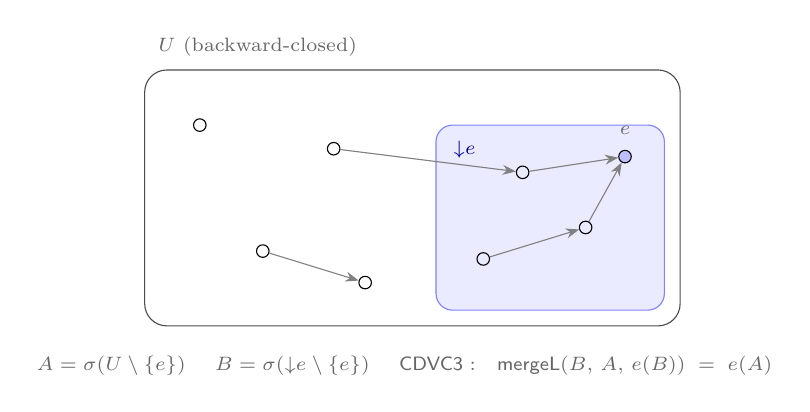
\begin{tikzpicture}[>=Stealth,
  ev/.style={circle, draw, inner sep=1.6pt, font=\scriptsize},
  lbl/.style={font=\scriptsize, text=black!60}]
% the big set U
\draw[rounded corners=8pt, black!70]
  (-0.4,-0.35) rectangle (6.4,2.9);
\node[lbl, anchor=south west] at (-0.35,2.95) {$U$ (backward-closed)};
% downset region
\begin{scope}[on background layer]
\fill[blue!8, rounded corners=6pt] (3.3,-0.15) rectangle (6.2,2.2);
\end{scope}
\draw[rounded corners=6pt, blue!50] (3.3,-0.15) rectangle (6.2,2.2);
\node[lbl, text=blue!60!black, anchor=north west] at (3.4,2.12) {$\dow{e}$};
% events
\node[ev] (x1) at (0.3,2.2) {};
\node[ev] (x2) at (1.1,0.6) {};
\node[ev] (x3) at (2.0,1.9) {};
\node[ev] (x4) at (2.4,0.2) {};
\node[ev] (y1) at (3.9,0.5) {};
\node[ev] (y2) at (4.4,1.6) {};
\node[ev] (y3) at (5.2,0.9) {};
\node[ev, fill=blue!25] (e) at (5.7,1.8) {};
\node[lbl, above=0.07cm of e] {$e$};
\draw[->, black!50] (y1) -- (y3);
\draw[->, black!50] (y2) -- (e);
\draw[->, black!50] (y3) -- (e);
\draw[->, black!50] (x3) -- (y2);
\draw[->, black!50] (x2) -- (x4);
\node[lbl] at (2.9,-0.85)
  {$A = \sigma(U\setminus\{e\})$ \quad
   $B = \sigma(\dow{e}\setminus\{e\})$ \quad
   $\cd:\ \ \mergeL(B,\, A,\, e(B)) \;=\; e(A)$};
\end{tikzpicture}
\caption{The causal-delta equation. The shaded region is $e$'s causal
past $\dow{e}$ (what $e$ saw); $e$ is $\loE{U}$-maximal. $e$'s effect on
the whole world $A$ equals: compute $e$'s effect on its own causal past
$B$, then merge that delta into $A$ \emph{over LCA $B$}. The merge sits at
its honest LCA: $(U\setminus\{e\}) \cap \dow{e} =
\dow{e}\setminus\{e\}$. Concurrent context that $e$ never observed
cannot amplify what $e$ does.}
\label{fig:cd}
\end{figure}

The update-side obligations of \S\ref{sec:join} and the merge-side laws
of \S\ref{sec:whydelta} now assemble into the full contract --- a
\emph{new} VC set, replacing the paper's catalogue of twenty-four. For
an MRDT $\langle \Sigma, \Sinit, \mathsf{do}, \mergeL,
\mathsf{rc}\rangle$, the contract is:

\paragraph{Update layer (unconditional, SMT-shaped).}
\begin{enumerate}[leftmargin=2.2em]
\item \textbf{rc-non-comm (guarded)} --- for distinct events \emph{from
  different replicas}: they fail to commute iff $\mathsf{rc}$ orders them
  in exactly one direction. \emph{The conflict table is the commutativity
  table, with a direction.} The different-replica guard is a semantic
  necessity, not a convenience: same-replica events are totally ordered
  by program order, so they are never concurrent and there is no
  conflict for $\mathsf{rc}$ to resolve. An unguarded VC would instead
  demand that $\mathsf{rc}$ order \emph{every} non-commuting pair ---
  unsatisfiable for real data types: the \emph{optimized OR-set}'s
  same-replica same-element adds do not commute (the newer add evicts
  the older tag), yet they can never race, and its $\mathsf{rc}$
  rightly ignores them. (The paper's F\textsuperscript{*} artifact
  carries exactly this guard in its interface ---
  \lean{App\_mrdt.fsti}: \texttt{requires distinct\_ops o1 o2
  /\char`\\\ get\_rid o1 <> get\_rid o2}.)
\item \textbf{no-rc-chain} --- conflict priorities do not chain: never
  $o_1 \rc o_2$ and $o_2 \rc o_3$. This is what makes the linearization
  order acyclic, so maximal events exist --- the entire peel-and-recurse
  architecture stands on it.
\item \textbf{cond-comm} --- a resolved conflict is invisible once an
  absorber runs: swapping an $\mathsf{rc}$-ordered concurrent pair deep in
  a fold changes nothing for any later non-commuting event, across
  arbitrary intervening events. This is the engine of convergence.
\end{enumerate}

\paragraph{Merge layer.}
\begin{enumerate}[leftmargin=2.2em]\setcounter{enumi}{3}
\item \textbf{merge symmetry} --- $\mergeL(l,a,b) = \mergeL(l,b,a)$.
\item \textbf{feasible unit} --- $\mergeL(\Sinit,\Sinit,\sigma(E)) =
  \sigma(E)$: merging over nothing is a no-op, on states that can arise.
\item \textbf{feasible local-redistribute} and
\item \textbf{feasible redistribute} --- Definition~\ref{def:delta},
  quantified over canonical tuples at honest LCAs.
\item \textbf{the causal-delta equation ($\cd$)} --- for a
  $\loE{U}$-maximal event $e$ of a backward-closed $U$, with
  $A = \sigma(U\setminus\{e\})$ and $B = \sigma(\dow{e}\setminus\{e\})$
  the canonical state of $e$'s own causal past:
  \[
    \mergeL\bigl(B,\; A,\; e(B)\bigr) \;=\; e(A).
  \]
  \emph{What an event does is determined by what it saw}
  (Figure~\ref{fig:cd}): applying $e$ to the whole world equals computing
  $e$'s delta on its causal past and merging it in over that past.
\end{enumerate}

Items 1--4 are one-liners for every data type we have discharged; items
6--7 frequently hold unconditionally anyway (for the OR-set,
\textsc{redistribute} is a pointwise Boolean tautology); essentially the
entire per-data-type proof effort concentrates in item 8, whose discharge
follows a uniform recipe: characterize $\sigma(E)$ (a ``sandwich''
invariant along canonical enumerations), then a \emph{trichotomy} placing
every event the maximal $e$ interacts with either inside $\dow{e}$ or
absorbed on a side that owns it.

Compare the published catalogue: 24~VCs per data type, plus five more the
soundness proof uses silently. Seventeen of the~24 --- the
\textsc{BottomUp} induction-scheme families --- exist to drive the broken
induction and are consumed nowhere in the corrected one; the paper's
\textsc{MergeIdempotence} is likewise never used. The seventeen were,
however, doing honest work of a different kind: they are an
\emph{automation layer}, Skolemizing ``holds on feasible states'' into
base-and-step equations an SMT solver can discharge. Rebuilding that
layer, aimed at the corrected target ($\cd$ rather than \textsc{BottomUp}),
is in our view the most valuable open engineering problem this work
leaves (\S\ref{sec:open}).

\section{Adequacy}
\label{sec:adequacy}

The contract delivers. Everything a data type owes is the eight
equations of \S\ref{sec:vcs}; everything else is proved once, for all
data types, as part of the execution model.

\begin{theorem}[soundness of the eight VCs]
\label{thm:main}
If an MRDT satisfies VCs 1--8, then every configuration reachable from
the initial configuration in the ternary transition system is
RA-linearizable, per version.
\hfill\lean{ra\_linearizable\_of\_core\_feasible\_cd3}
\end{theorem}

The proof shape: the update layer powers the set-relative convergence
theorem, hence canonical states; the transition induction maintains
``every store version is canonical for its event set'' (fork and query
are trivial; apply is the extend lemma); the merge case reduces, via
Lemma~\ref{lem:lca}, to the ternary Join Lemma, which is proved from VCs
4--8 by strong induction on $|E_1 \cup E_2|$: select a
$\loE{E_1\cup E_2}$-maximal $e$, decompose each side containing $e$
through $\dow{e}$ (\textsc{local-redistribute} at the honest LCA
$\dow{e}\setminus\{e\}$), cancel the shared delta
(\textsc{redistribute}), close the principal step with $\cd$, and recurse.
The buried-event pathology of Example~\ref{ex:defeater} dissolves
structurally: no step ever asks how a \emph{side's} state factors ---
every factoring happens through the join.

Everything else one might fear owing is proved once, for all data types,
as an execution-model invariant: visibility transitivity, per-version
backward closure, store well-formedness, and Lemma~\ref{lem:lca} itself.
The data type owes exactly the eight equations.

\paragraph{A second route, and an honest asymmetry.} One discharged data
type does not fit the pattern above. The enable-wins flag's merge
\emph{compares counters} against the LCA, and for such merges the Join
Lemma's hypotheses as stated (backward closure under
non-commuting-visibility) are provably too weak: there is a
closure-legal tuple --- a live LCA enable, a dead post-LCA enable
inflating one side's counter, the killing disable visible only to the
other side --- on which the production merge computes the wrong flag. Full
\emph{causal} closure (which the store invariant actually supplies)
excludes it, and the flag is discharged through a full-closure variant of
the join. The finding: \textbf{required closure strength is a function of
the merge's shape} --- commutation-closure suffices for set-shaped merges,
counter-comparison merges need full causal closure. Reunifying the two
routes was expected to be routine --- ``full closure only strengthens what
a data type may assume.'' Mechanization shows it is not (\S\ref{sec:open},
Open Question~\ref{oq:reunify}): the naive reunification --- re-run the
Join Lemma induction with full-closure hypotheses --- is refuted, because
no single-event (or block) peel preserves full closure. What survives is a
\emph{closure-indexed} contract in which the data type \emph{declares} its
closure strength; the soundness bridge is uniform across strengths, so no
reunification into one strength is needed.

\section{The catalogue, discharged}
\label{sec:catalog}

\begin{table}[t]
\centering
\footnotesize
\resizebox{\textwidth}{!}{%
\begin{tabular}{@{}llll@{}}
\toprule
MRDT & contract tier & end-to-end theorem & $\sigma$-characterization (one line) \\
\midrule
Grow-only set & unconditional & \lean{GOSet\_ra\_linearizable3\_eq} & union of adds \\
Grow-only map & unconditional & \lean{GOMap\_ra\_linearizable3\_eq} & union of $(k,v)$ records \\
Incr.-only counter & unconditional & \lean{IOC\_ra\_linearizable3\_eq} & $\#$events \\
PN-counter & unconditional & \lean{PN\_ra\_linearizable3\_eq} & $\#\mathsf{inc}-\#\mathsf{dec}$ \\
RGA (tombstone) & unconditional & \lean{RGAM\_ra\_linearizable3\_eq} & grow-only nodes + tombstones \\
Peritext & unconditional & \lean{Peritext\_ra\_linearizable3\_eq} & grow-only mark records \\
OR-set & feasible & \lean{ORSet\_ra\_linearizable3\_eq} & tag live iff added, no vis-later $\rem$ \\
OR-set (efficient) & feasible & \lean{ORSetE\_ra\_linearizable3\_eq} & \dots{} or same-replica $\add$ later (eviction) \\
Enable-wins flag & full-closure & \lean{EWFlag\_ra\_linearizable3\_eq} & per key: ctr $=\#$enables; flag iff unkilled enable \\
\midrule
Multi-valued register & feasible & \lean{MVR\_ra\_linearizable3\_eq} & tagged writes $\times$ overwrite log; all-comm $\Rightarrow B{=}\Sinit$ \\
Add-wins priority queue & feasible & \lean{AWPQ\_ra\_linearizable3\_eq} & the OR-set pattern on A; grow-only I \\
Bounded counter (escrow) & all-comm & \lean{BC\_ra\_linearizable3\_eq} & convergence flat; the \emph{bound} is a conditioned safety theorem (\lean{bc\_version\_inv}) \\
FWW reservation register & all-comm & \lean{FWW\_ra\_linearizable3\_eq} & payload arbitration (min-ts semilattice); winner characterized at every version (\lean{fww\_version\_min}) \\
LWW register & all-comm & \lean{LWW\_ra\_linearizable3\_eq} & payload arbitration (max-ts semilattice), the last-writer twin of FWW; winner characterized (\lean{lww\_version\_max}); \emph{end-to-end mechanized}, unlike the flat CRDT LWW (sorry-carrying VC bridge) \\
BudgetCart & or-set $\rc$ & \lean{BCart\_ra\_linearizable3\_eq} & budgeted cart, spend derived from live instances; safety \emph{gated} on causal canonicity (OQ~\ref{oq:causalcanon}) \\
Mergeable queue (Peepul) & \emph{direct join} & \lean{queue\_ra\_linearizable3} & no $\rc$ exists (enqueue clique); the merge itself is the linearization witness \\
RGA (tombstone-free) & \emph{conditioned} & \multicolumn{2}{l}{\lean{rga\_tombstone\_free\_ra\_linearizable3\_eq} --- RA-lin up to $\approx$, honest delivery (\S\ref{sec:open})} \\
Peritext (tombstone-free) & \emph{composed} & \multicolumn{2}{l}{\lean{peritextComposed\_ra\_linearizable\_up\_to\_eq} --- RGA${}\otimes{}$marks through the product kit; 1{,}064 lines total} \\
Peritext (tombstone-free, fused) & \emph{fused} & \multicolumn{2}{l}{\lean{peritext\_ra\_linearizable\_up\_to\_eq} --- one RGA at $\alpha := \mathsf{char} \oplus \mathsf{boundary}$; convergence by instantiation, genuine positional intent (\lean{render\_id\_active\_iff\_between}); 773 lines} \\
\bottomrule
\end{tabular}}
\caption{The Sal production catalogue. Every instance concludes through
the ONE generic conditioned metatheorem
(\S\ref{sec:condmeta}--\S\ref{sec:actual}): the nine flat data types at
the identity instantiation ($\eqobs = {=}$, their VC bundles feeding the
flat collapse \lean{FlatGeneric\_Bridge.lean}, instance theorems in
\lean{MRDT\_Instances/ (per-RDT)}), the tombstone-free RGA at full
generality. The contract-tier column is each data type's Join-Lemma
discharge content (\lean{MRDT\_Instances/}, one directory per RDT); the historical flat
corollaries over the raw system remain there as internal steps.}
\label{tab:catalog}
\end{table}

Table~\ref{tab:catalog} is the empirical heart of the note: the VC set is
not merely adequate in principle --- the data types people actually ship
satisfy it. Three lessons from the sweep:

\paragraph{Tombstones are a metatheoretic trivializer.} The catalogue's
celebrated hard cases --- the RGA sequence type and the Peritext
rich-text type --- land in the \emph{easiest} tier. The reason is almost
embarrassing: with tombstones, deletion \emph{adds} a record; every state
component is grow-only; all operations commute; the merge is a blind
join. All of the RGA's genuine difficulty lives in the \emph{read-side}
traversal (turning the node soup into a sequence), which
RA-linearizability of the state never touches. By contrast the
\emph{tombstone-free} RGA --- which physically deletes and repairs
positions by climbing ancestor paths --- is the one data type the eight
VCs cannot host, for a reason worth stating precisely: its commutation VC
is itself \emph{reachability-conditioned} (two inserts commute only on
well-formed states), and the update layer above, like the paper's,
quantifies over all states. That was the question the tombstone-free RGA
was built to force, and it is now answered --- not by a conditioned
update \emph{layer} (every layer-level conditioning is refuted, see the
feasible-update question in \S\ref{sec:open}) but by a conditioned
\emph{metatheory} that abandons pointwise swaps altogether; the resulting
end-to-end theorem is RA-linearizability up to observational equivalence
under honest delivery.

\paragraph{Commutation class and delta class are independent axes.} The
multi-valued register is all-commuting, yet \emph{not} in the
unconditional tier: its merge is intersection-shaped,
$(l \cap a \cap b) \cup (a \setminus l) \cup (b \setminus l)$, and fails
the delta laws on infeasible tuples exactly as the OR-set does. The
boundary between tiers is drawn by \emph{how the merge uses its LCA}, not
by whether operations commute. (The compensation: all-commuting makes
every punctured causal past empty, $B = \Sinit$, so the feasible
discharge needs no trichotomy at all.)

\paragraph{The eight VCs certify real code on its historical fault
line.} The enable-wins flag's repository history contains a
known-broken sibling: a global-counter variant whose compositional VC
(\lean{inter\_right\_1op}) fails on DAG-shaped executions, the very defect
per-replica counters were introduced to fix. The mechanized $\sigma$-facts
prove the production merge computes exactly union-liveness ---
\emph{verified on precisely the corner where the sibling fails}. This is
the methodology working as intended: the metatheory does not merely bless
the catalogue, it explains \emph{why} the fixed design is right.


\section{The conditioned metatheorem}
\label{sec:condmeta}

The eight VCs of \S\ref{sec:vcs} quantify over \emph{all} states, and
\S\ref{sec:catalog} showed that is right for flat data types and fatal
for state-dependent ones: in the tombstone-free RGA of
\S\ref{sec:mrdts}, two concurrent inserts commute only when each one's
anchor is faithfully resolvable in the other's presence, and an insert
under a since-deleted, physically-removed node is not even applicable.
Written over all states, the commutation VC is simply false (a mechanized
counterexample: \lean{naive\_general\_swap\_false}). The remedy is the
general signature of \S\ref{sec:mrdts}: condition every VC on the state
invariant $\Inv$ and the applicability predicate $\app$, relax the
witness fold of Definition~\ref{def:ralin} to the data type's
observational equivalence $\eqobs$, and prove RA-linearizability from the
conditioned VCs once and for all. The developer's burden is only to
describe sensible operations; the metatheorem does the rest. This section
states the conditioned VCs and the metatheorem with its pen-and-paper
proof; \S\ref{sec:rgaend} discharges the VCs for the tombstone-free RGA;
\S\ref{sec:actual} records how the mechanization actually went ---
including the machine-checked refutations that reshaped the route --- and
what the completed assembly proves.

\section{The conditioned verification conditions}\label{sec:cvcs}

A datatype presents a signature
$\langle \text{State}, \ini, \dodo, \merge, \Inv, \app \rangle$ where $\Inv$ is a predicate
on states and $\app$ a predicate on (operation, state) pairs (Lean:
\lean{ConditionedMRDTSig}, \lean{Framework/MRDTSig.lean}). It must supply:

\begin{vc}[Discipline]\label{vc:disc}
$\Inv\,\ini$ holds; $\dodo$ preserves $\Inv$ on applicable operations; and generation is
disciplined: every operation is $\app$ and \emph{fresh} at its birth state, with globally
unique, monotone ids. (This is the execution model, Lean:
\lean{ConditionedConfiguration}, \lean{Framework/ConditionedExecutionModel.lean} --- kernel-clean,
axiom-free.)
\end{vc}

\begin{vc}[Conditioned commutation --- the swap witness]\label{vc:comm}
For concurrent operations $a,b$ and any state $\st$ with $\Inv\,\st$ at which both are
applicable in the relevant reorder sense, $\dodo\,(\dodo\,\st\,a)\,b \eqobs
\dodo\,(\dodo\,\st\,b)\,a$.
\end{vc}

\begin{vc}[Threadable reorder invariant]\label{vc:inv}
An auxiliary invariant $J$ on (state, pending-event) that (i) certifies applicability/the
swap precondition of VC~\ref{vc:comm} at reorder states, (ii) holds at the enabling fold of
each event, and (iii) is preserved by each reorder step. Only the \emph{enabled} events ---
those whose causal past is folded --- need be certified; that scope is exactly what a
linearization repair ever transposes.
\end{vc}

\begin{vc}[Merge--linearization bridge --- the conditioned Join Lemma]\label{vc:merge}
For a reachable LCA state $l$ and branches $a,b$ obtained from $l$ by disjoint concurrent
event lists, $\merge\,l\,a\,b \eqobs \fold\,l\,\pi$ for a $\loE{E}$-respecting enumeration $\pi$
of the branch events.
\end{vc}

For flat datatypes $\Inv = \app = \mathsf{true}$, VC~\ref{vc:comm} degenerates to
unconditioned commutation, VC~\ref{vc:inv} to $J = \mathsf{true}$, and VC~\ref{vc:merge} to
the ordinary Join Lemma --- recovering the unconditioned methodology.

\section{The metatheorem}\label{sec:meta}

\begin{theorem}[Soundness --- conditioned VCs $\Rightarrow$ RA-linearizability]\label{thm:meta}
Any MRDT satisfying VCs~\ref{vc:disc}--\ref{vc:merge} is RA-linearizable
(Definition~\ref{def:ralin}, read up to $\eqobs$).
\end{theorem}

The proof is generic --- it never inspects a particular datatype --- and factors through two
lemmas, each proved over the abstract signature with $\eqobs$ an arbitrary congruence for
$\dodo$ and $\merge$.

\begin{remark}[Route actually taken]
The convergence lemma below is stated via the swap-based VC~\ref{vc:inv} for exposition. That
route is \emph{machine-refuted} for the tombstone-free RGA; convergence is mechanized by direct
canonical-state characterization instead. See Section~\ref{sec:actual}.
\end{remark}

\begin{lemma}[Convergence]\label{lem:conv}
VCs~\ref{vc:disc},~\ref{vc:comm},~\ref{vc:inv} imply that all $\loE{E}$-respecting admissible
enumerations of a backward-closed reachable $E$ fold from $\ini$ to $\eqobs$-equal states;
hence $\sigmacan(E)$ is well defined up to $\eqobs$.
\end{lemma}
\begin{proof}
Any two $\loE{E}$-respecting enumerations of $E$ are related by repeatedly transposing adjacent
$\loE{E}$-incomparable events. Because $\loE{E}$ is non-transitive, ``respecting'' is the elementwise
\lean{Pairwise} condition rather than sortedness, so this order-repair is more delicate than
for a total order --- it is exactly what the generic engine \lean{eq\_convergence} carries out,
and we appeal to it rather than re-derive it. Each transposition preserves the fold up to
$\eqobs$ by VC~\ref{vc:comm}, provided the swap precondition holds at the transposition point;
VC~\ref{vc:inv} supplies it along the whole enumeration (base at each event's enabling fold,
preserved by each step, scoped to the enabled events --- the only ones the repair transposes).
The engine consumes only that $\eqobs$ is an equivalence, $\dodo$ is $\eqobs$-congruent, and a
swap oracle of the shape VC~\ref{vc:comm}$+$\ref{vc:inv} provides (Lean: \lean{eq\_convergence},
kernel-clean).
\end{proof}

\begin{lemma}[Canonical adequacy]\label{lem:adeq}
VC~\ref{vc:merge} and Lemma~\ref{lem:conv} imply that every reachable version state is
$\eqobs\ \sigmacan$ of its delivered event set.
\end{lemma}
\begin{proof}
Induction over the version DAG. Initial: the empty fold. Update node: appends one delivered
operation to a canonical fold (definitional). Merge node with LCA $l$ and branches $a,b$: by
hypothesis $a \eqobs \sigmacan(E_a)$ and $b \eqobs \sigmacan(E_b)$, and $l \eqobs
\sigmacan(E_l)$. First rewrite $a,b$ to literal canonical folds using $\eqobs$-congruence of
$\merge$ (so VC~\ref{vc:merge}, stated for branch folds, applies); then VC~\ref{vc:merge}
gives $\merge\,l\,a\,b \eqobs \fold\,l\,\pi$ for a $\loE{E}$-respecting $\pi$ of the branch
events $E_a \cup E_b$. Now $E_l$ causally precedes those branch events (they were generated on
states derived from $l$), so a $\loE{E}$-respecting enumeration of $E_l \cup E_a \cup E_b$
factors as (an $\loE{E}$-enumeration of $E_l$) followed by $\pi$; hence
$\fold\,l\,\pi = \fold\,(\sigmacan(E_l))\,\pi \eqobs \sigmacan(E_l \cup E_a \cup E_b)$ by
Lemma~\ref{lem:conv} (the engine is start-state generic). Backward closure keeps every
enumeration admissible.
\end{proof}

\begin{proof}[Proof of Theorem~\ref{thm:meta}]
Immediate from Lemma~\ref{lem:adeq}: each version state $\eqobs \sigmacan(E_v)$, which is
Definition~\ref{def:ralin}. (Unconditioned template: \lean{ra\_linearizable3\_of\_joinC} plus
the closure-indexed adequacy bridge, already kernel-clean with nine instances; the
conditioned metatheorem generalizes it by carrying $\Inv/\app$ through the two lemmas.)
\end{proof}

\begin{corollary}[Strong eventual consistency]\label{cor:sec}
Two versions with the same delivered set $E$ have $\eqobs$ states: both $\eqobs \sigmacan(E)$
by Theorem~\ref{thm:meta}, hence $\eqobs$ each other.
\end{corollary}

\section{The tombstone-free RGA discharges the conditioned VCs}\label{sec:rgaend}

The RGA is a forest of identified nodes; $\dodo$ inserts a fresh node under a resolved anchor
or physically deletes a node and rehomes its children; $\merge$ keeps OR-set survivors and
re-anchors each by climbing to the nearest surviving ancestor. $\resolve\,\st\,p$ returns the
first live id on a recorded path $p$; $\anc\,\st\,x$ is $x$'s current parent. Take
$\Inv := \mathsf{wf} \wedge \mathsf{id\_mono} \wedge (\text{root not reinserted})$ and
$\app := \mathsf{accurate} \wedge \mathsf{fresh}$. This section presents the discharge as
it was \emph{first attacked}: swap-based, with the two hard VCs reduced to one faithfulness
invariant.

\paragraph{First, the evidence that the flat schema is out of reach.} The
introduction's claim that this data type is \emph{provably outside} the flat
VC set rests on two kernel-checked refutations at the $\dodo$ level, one per
escape route (the visual account, with the traces drawn, is
\lean{Sal/MRDTs/RGA\_Rehoming/doc/why-the-path-matters.pdf}, \S6).
\emph{Route one: no path.} The path-free splice predecessor
(\lean{RGA\_Splice}, branch \lean{wip/rga-splice}) has
$\mathsf{Ins}(t\ \text{after}\ x)$ and $\mathsf{Del}(x)$ genuinely
non-commuting (the splice destroys the parent pointer), so the flat schema's
commutation iff (\lean{rc\_non\_comm}) forces the entry
$\mathsf{rc}(\mathsf{Ins}(t\ \text{after}\ x), \mathsf{Del}(x)) =
\mathsf{Fst\_then\_snd}$ --- and a non-Either entry awakens the
conditional-commutation base VC (\lean{cond\_comm\_base}: an
$\mathsf{rc}$-ordered pair must be order-insensitive at application whenever
a third op also conflicts), which the three-operation trace
$\mathsf{Ins}(10\ \text{after}\ 5);\mathsf{Del}(5);
\mathsf{Ins}(12\ \text{after}\ 5)$ from $\{(5,\cdot,0)\}$ refutes: the first
insert is rehomed onto the root in the mandated order but dangles in the
flipped one (\lean{cond\_comm\_base\_violated}, by evaluation).
\emph{Route two: the path.} Carrying the ancestor path repairs exactly that
trace (\lean{trio\_converges}) but the repaired commutation is
\emph{reachability-conditioned}: the mechanized \lean{rc\_non\_comm'}
assumes the carried paths are \lean{accurate} in the state, and dropping
that hypothesis is refuted by a lying record ---
$\mathsf{Ins}(10\ \text{after}\ 5, \langle 7\rangle)$ accurate against
$\mathsf{Del}(5, \langle\rangle)$ claiming $5$ hangs off the root; whichever
runs second applies \emph{its own} record and the orders diverge
(\lean{inconsistent\_diverges}). Accuracy is a property of the execution
that generated the operation, not of the state it meets, so no
$\forall\sigma$ equation can carry it: the schema cannot be satisfied, only
\emph{changed} --- which, done soundly, is the conditioned framework of
\S\ref{sec:condmeta}.

\begin{definition}[Recorded-path faithfulness $\RVF$]\label{def:rvf}
$\RVF\,a\,\st$: the recorded path $\recList\,a$ is a \emph{live subchain of genuine
ancestors} of $a$'s target in $\st$ --- true $\anc$-ancestors, nearest first, consecutive
pairs real parent edges, and exactly the chain live at $a$'s generation. (This is
\lean{accurate}/\lean{HistFaithful} promoted to a reachability invariant.)
\end{definition}

\begin{lemma}[$\RVF$ is a reachability invariant]\label{lem:rvf}
$\RVF\,a\,\st$ holds at every reachable $\st$ in which $a$ is applied.
\end{lemma}
\begin{proof}
Induction on the operations building $\st$. \emph{Birth:} $\dodo$ sets
$\recList\,a = \resolve\text{-path}$ at generation $=$ the live-ancestor chain, so $\RVF$
holds (\lean{chainFaithful\_of\_histFaithful}). \emph{Later $\mathsf{Ins}$ with fresh id
$f$:} attaches $f$ as a descendant --- no reparenting, no liveness change for prior events'
chains. $f$ cannot appear spuriously in any $\recList\,a$: its members are older ids
$< a.\mathsf{id} \le$ every id extant at $a$'s birth, whereas $f$ exceeds all of them, so
$f \notin \recList\,a$ definitionally. The resurrection/clash regime
(\lean{chainFaithful\_not\_preserved\_under\_clash\_ins}) is therefore \emph{unreachable} by
freshness (\lean{fresh\_not\_mem\_recList}, \lean{clash\_recList\_excluded}), not excluded by
a side condition. \emph{Later $\mathsf{Del}\,x$:} flips $x$'s liveness only; $\recList\,a$'s
entries stay genuine ancestors, one possibly now dead --- still a live subchain
(\lean{chainFaithful\_doDel\_faithful}).
\end{proof}

\begin{lemma}[Key Lemma: resolution over a live subchain]\label{lem:key}
For any live subchain of genuine ancestors $pre$ of $x$, in every reachable $\st$,
$\resolve\,\st\,pre = \anc\,\st\,x$. (Lean: \lean{subchain\_resolve},
\lean{RGA\_SubchainResolve.lean}, kernel-clean.)
\end{lemma}
\begin{proof}
$\resolve$ returns the first entry live in $\st$; each entry is a genuine ancestor, so this is
the nearest live ancestor among $pre$. It is the nearest overall: no live ancestor $c \notin
pre$ is nearer than that first-live entry --- (a) if $c$ was live at capture it was in the
captured live chain, so $c \in pre$ (and any $pre$-entry nearer than the first-live one is
dead in $\st$, hence not $c$); (b) if $c$ was dead at capture it is still dead (physical,
tombstone-free deletion is permanent); (c) an event inserted after capture attaches as a
descendant, never a new ancestor of the pre-existing $x$. The mechanization absorbs these
three cases into one preserved invariant
$\mathsf{LiveChain}\,\st\,x\,pre := (\text{root unstored}) \wedge \contains\,\st\,x \wedge
\mathsf{IsAncPath}\,\st\,x\,(pre.\mathsf{filter}\,\contains)$, which holds at capture, is
preserved by each insert (\lean{isAncPath\_upd}) and delete (\lean{isAncPath\_surgery}, chain
splicing across a deleted entry), and yields the conclusion. Case~(b) is discharged by an
explicit hypothesis $t \notin pre$ on inserts (\lean{okStep}) --- the mechanized form of ``no
resurrection,'' itself a consequence of monotone allocation, every $pre$-entry sitting below
$x$'s id. This replaces the earlier full-chain lemma \lean{hres\_of\_lchain}, which failed on
the proper subchains rehoming produces.
\end{proof}

\begin{proposition}[RGA discharge]\label{prop:discharge}
The RGA satisfies VCs~\ref{vc:disc}--\ref{vc:merge}. (Proof sketch below along the swap route; in the final
mechanization the \emph{entire} route --- the swap VC, the $\ChainFaithful$ threading, the
per-id $\mathsf{BranchInv}$ --- is superseded by the canonical-state engine of
Section~\ref{sec:actual}, and only the Key Lemma survives; see the audit note there.)
\end{proposition}
\begin{proof}
\emph{VC~\ref{vc:disc}} (discipline): $\Inv$ preservation and the generation model are
\lean{ConditionedConfiguration} instantiated at the RGA, with the RGA's $\dodo$-invariance
lemmas; \lean{conditioned\_premises} supplies the timestamp/freshness facts.
\emph{VC~\ref{vc:comm}} (swap): \lean{general\_swap\_bothFaithful} /
\lean{eqSwap\_of\_bothFaithful} --- concurrent operations commute up to $\eqobs$ when both
are \emph{faithful} (neither need be exact/accurate), kernel-clean.
\emph{VC~\ref{vc:inv}} (reorder invariant): $J := \ChainFaithful$ on the enabled scope, with
steps \lean{chainFaithful\_incompStep}/\lean{incompFold}; its \emph{base} --- each event
faithful at its enabling fold --- is exactly $\RVF$ (Lemma~\ref{lem:rvf}) projected through
the Key Lemma (Lemma~\ref{lem:key}): the residual goal
$\resolve\,\st\,((\recList\,a)\setminus t') = anch'$ when an ancestor $t'$ becomes leftmost
live is the Key Lemma on the remaining subchain.
\emph{VC~\ref{vc:merge}} (Join): per-id extensional match
(\lean{eq\_merge2\_of\_branchInv2}); the anchor-coincidence clause is the single-sided
$I_4$ (\lean{eq\_merge\_single}, kernel-clean) and, cross-branch, the Key Lemma directly
(\lean{branchInv\_doDel\_crossBranch}, kernel-clean); order-independence is Lemma~\ref{lem:conv}
at start state $l$. (In the final assembly this per-id $\mathsf{BranchInv}$ threading is
itself superseded by the birth-anchor bridges of Section~\ref{sec:actual}, which need no
invariant threading at all.)
Both hard VCs (\ref{vc:inv} base, \ref{vc:merge} cross-branch) thus rest on $\RVF$ and the
Key Lemma --- proved by construction from freshness and permanence.
\end{proof}

\begin{corollary}
The tombstone-free RGA is RA-linearizable (Theorem~\ref{thm:meta} + Proposition~\ref{prop:discharge}),
and strongly eventually consistent (Corollary~\ref{cor:sec}). To our knowledge this is the
first mechanized RA-linearizability / SEC result for an RGA with physical, tombstone-free
deletion (cf.\ Gomes et al., OOPSLA'17, for the tombstoned RGA).
\end{corollary}

\begin{remark}[Other instances]
The nine flat production MRDTs (counter, OR-set, MVR, \dots) take $\Inv=\app=\mathsf{true}$:
VC~\ref{vc:comm} is their unconditioned commutation, VC~\ref{vc:inv} is $J=\mathsf{true}$,
and VC~\ref{vc:merge} is the ordinary Join Lemma --- already discharged
(\lean{ra\_linearizable3\_of\_joinC}). They inherit RA-linearizability from the same
Theorem~\ref{thm:meta}. The RGA is the instance that exercises every conditioned mechanism;
the framework supplies the generality, the RGA the novelty.
\end{remark}

\section{How it was actually mechanized (and two dead ends)}\label{sec:actual}

The exposition above (Sections~\ref{sec:vcs}--\ref{sec:rga}) is the \emph{intended} route, and it
correctly frames the contribution: conditioned VCs $\Rightarrow$ RA-linearizability, RGA as
instance. But the mechanization did \emph{not} follow the swap-based convergence of
VC~\ref{vc:inv}. That route was tried and \textbf{machine-refuted twice}; convergence was then
proved by a different technique. We record the actual route honestly --- the refutations are
themselves findings about why tombstone-free deletion is hard.

A postscript, established after the assembly was complete: a kernel-level dependency audit of
the capstone's compiled proof term shows the subsumption is \emph{total}. The final theorem's
dependency cone contains no swap lemma, no $\ChainFaithful$/$\RVF$ threading, and no
$\mathsf{BranchInv}$ --- of the swap route only the Key Lemma remains load-bearing. The
route's files stay proved and kernel-clean, retired under \lean{Development/}; of the
investigation's ${\sim}17$k lines, the capstone's dependency cone spans ${\sim}8$k. The
lesson generalizes the refutations: for a datatype whose operations reference mutable
structure, the set-indexed characterization is not just an alternative to
linearize-and-swap --- it makes the swap layer unnecessary even where the swaps are
provable.

\paragraph{Two machine-checked refutations of the swap route.} The reorder-invariant convergence
(VC~\ref{vc:inv}, ``thread faithfulness through adjacent swaps'') fails for the tombstone-free
RGA because \emph{rehoming makes an event's recorded chain time-relative}: correct at generation,
wrong at reordered intermediate states.
\begin{itemize}[nosep]
  \item \textbf{$\loE{E}$ is not transitive} (\lean{RGA\_DepComp\_Gate}, kernel-clean refutation).
  Reordering dependencies-contiguous-first needs transitivity of the linearization order; a
  physical delete severs an operation's applicability-dependence on an ancestor
  ($b\!\to\!a\!\to\!o$ but $\neg(b\!\to\!o)$ after $a$'s target is deleted). Witness:
  $l=0\!\leftarrow\!1\!\leftarrow\!2\!\leftarrow\!3$, delete node~1, delete node~2.
  \item \textbf{In-place threading fails at the ancestor-insert step}
  (\lean{RGA\_SimulInduction2}, kernel-clean refutation). Even threading without reordering, an
  event's recorded chain can be \emph{ahead} of the state (it anticipates a delete not yet folded),
  so $\ChainFaithful$ of the recorded chain is false at that intermediate fold although it heals
  later.
\end{itemize}
Both say the same thing: the linearize-and-swap method, which needs faithfulness at every
\emph{intermediate} reordered state, is the wrong vehicle. This is exactly what tombstones prevent
(Gomes et al.\ keep deleted nodes so dependencies never rewire); the tombstone-free RGA rewires
them.

\paragraph{The technique that works: direct canonical-state characterization.} Instead of swaps,
characterize the fold state as a pure function of the applied event \emph{set} --- the update
analog of the merge bridge (which always worked). For a finite applied set $F$, define
$\mathsf{survivors}\,F$ (OR-set survival) and $\mathsf{canonAnc}\,F\,k$ (climb $k$'s recorded chain
to the nearest survivor of $F$); let $\mathsf{CanonMatch}\,F\,s$ say $s$ matches this per id.
\begin{lemma}[Canonical fold]\label{lem:canon}
Along any $\loE{E}$-respecting enumeration $\pi$, $\mathsf{CanonMatch}\,(\pi\text{-applied})\,
(\fold\,\ini\,\pi)$ (Lean: \lean{canon\_fold}, kernel-clean). Two folds of the same $E$ then both
match $\mathsf{CanonMatch}\,E$, hence are $\eqobs$ --- convergence with no swaps and no
intermediate-state faithfulness (\lean{RGA\_update\_convergence\_canon}; discharged from the
per-event generation discipline $\mathsf{GenDisc2C}$ in \lean{RGA\_update\_convergence\_final}).
\end{lemma}
The invariant is over the \emph{applied} set, so $\mathsf{canonAnc}\,F$ never anticipates a future
delete --- exactly why it succeeds where the swap route (which reasons about not-yet-applied
events) fails. The Key Lemma (Lemma~\ref{lem:key}) survives unchanged as the per-id climb-vs-resolve
coincidence; $\RVF$ is subsumed by $\mathsf{CanonMatch}$'s per-survivor \lean{LiveChain}.

\paragraph{The metatheorem as a generic $\eqobs$-quotient functor.} Theorem~\ref{thm:meta} is
mechanized generically over \lean{ConditionedMRDTSig} (\lean{RA\_linearizable\_up\_to\_eq},
\lean{GenericEqQuotient}, kernel-clean). It quotients the state by $\eqobs$ over the $\Inv$-subtype
and transfers the datatype's $\eqobs$-Join to the structural-$=$ template
\lean{ra\_linearizable3\_of\_joinC} by \lean{Quotient.sound}; the readback is over \emph{raw}
$\fold$, matching the RGA's convergence. The datatype supplies five VCs: $\mathsf{EqEquiv}$,
$\mathsf{InvPres}$, $\mathsf{CongVC}$ (update/merge/query $\eqobs$-congruent on $\Inv$),
$\mathsf{InvInvVC}$, and the $\eqobs$-Join $\mathsf{EqJoinLemma3C}$. Two subtleties the
mechanization forced, each machine-verified:
\begin{itemize}[nosep]
  \item \textbf{The merge $\eqobs$-congruence is false on the full state type}
  (\lean{merge\_eq\_congr\_l\_fails}, axiom-free), true on the reachable subfamily
  ($\mathsf{wf}\wedge\mathsf{id\_mono}\wedge\text{forest}$): the LCA-climb reads $\anc\,l$ off
  $\mathsf{domain}\,l$, where $\eqobs$ is silent. Hence the $\Inv$-conditioning of $\mathsf{CongVC}$
  is load-bearing, and the quotient is over the $\Inv$-subtype (\lean{merge\_eq\_congr\_inv}).
  \item \textbf{Invariant preservation needs well-formedness, not applicability.} $\mathsf{InvPres}$
  cannot demand unconditional preservation ($\dodo$ at a bad id breaks the invariant), nor full
  $\app$ (which the execution model does not guarantee --- \lean{Step3.apply} applies with only
  timestamp freshness). The honest condition is a datatype predicate $\mathsf{WfOp}$ (for the RGA:
  fresh id for $\mathsf{Ins}$; $\resolve\,s\,p \neq x$ for $\mathsf{Del}\,p\,x$), preserved by the
  real $\dodo$ (\lean{rgaInv\_doOp\_fresh}, accuracy \emph{removed}) and holding along reachable
  folds ($\mathsf{WfOpReachable}$). A totality guard on the lifted step is provably transparent on
  the execution domain ($\mathsf{applySeqW}=\mathsf{applySeq}$); the exposed theorem is over the
  real $\dodo$.
\end{itemize}

\paragraph{The completed assembly.} Everything after the quotient functor was, at the
first writing of this note, ``bounded assembly.'' Carrying it out surfaced three further
machine-checked refutations that reshaped the target and the witness discipline; we record
them because each is a fact about tombstone-free deletion, not about our proof.

\begin{itemize}[nosep]
  \item \textbf{At a merge union, applicability-tolerant witnesses do not exist.} An
  LCA-first enumeration pre-applies one branch's anchor-killing deletes before replaying the
  other branch's inserts, staling their recorded paths --- so even \emph{no-op-feasible}
  witnesses (each step applicable or a no-op) are unsatisfiable from the initial state
  (\lean{RGA\_HEnum\_Refutation}). Worse, on a seven-event two-branch execution \emph{no}
  born-applicable enumeration of the union replays both branches' recorded observations:
  rehoming makes the \emph{order of concurrent deletes} observable in survivors' stored
  parents, and the branches observe it differently. Consequently the linearization target
  itself must be the \emph{raw} $\dodo$-fold, up to $\eqobs$ --- any guarded or
  feasibility-filtered fold is unsatisfiable at merge unions
  (\lean{IsRALinearizable3Eq}, \lean{GoodConfig3H.lean}).
  \item \textbf{The witness discipline is the engine's own, plus payload honesty.} Each
  version carries, existentially, an enumeration satisfying the canonical engine's per-step
  discipline (\lean{CanonFoldOK}: fresh nonzero ids, no id reuse, live recorded chains)
  \emph{and} payload honesty (\lean{HonestPayloads}: delete targets and recorded-chain
  entries are root-or-inserted). The second clause is forced by a counterexample: the fold
  discipline alone admits a dead-target delete (a no-op), and a later insert reusing that
  recorded dead id breaks the no-id-reuse clauses --- honesty of \emph{payloads} is
  set-level, hence permutation-invariant, and it is exactly what extension at a fresh apply
  needs (\lean{rga\_hHext\_discharged}). The discipline \emph{joins} at merges with the
  union witness being the LCA-then-delta concatenation $\rho_0 +\!\!+\, \pi_0$ itself:
  no reordering, no swaps, anywhere (\lean{rgaJoinH\_of\_canon}).
  \item \textbf{The generation discipline is derived, not assumed.} Every event is
  accurate at the fold of its \emph{transitive dependencies} (\lean{GenDisc2C}), provable
  from \emph{born accuracy} --- the op was generated against a causal fold of the events its
  replica had seen (\lean{genDisc2C\_of\_born}). Merge canonicity then reduces to three
  leaves, all discharged: $\sigma_0$ id-monotonicity with \emph{no fold induction} (the
  stored anchor is $\mathsf{canonAnc}$ of the recorded chain, whose entries are
  dependencies, which are Lamport-below --- \lean{rga\_Hdec\_discharged}); a per-id causal
  set-algebra whose only non-trivial clauses are dependency-fold provenance
  (\lean{rga\_hcaus\_discharged}); and per-survivor \emph{birth-anchor bridges} reducing
  the merged forest's anchors to record coherence at dependency folds, where the generation
  discipline makes every recorded chain live
  (\lean{rga\_hbridge\_discharged}, \lean{hin\_of\_genDisc}).
\end{itemize}

The residual, quantified once over the execution, is a single per-step assumption
(\lean{HonestDelivery}): \emph{born accuracy} plus \emph{born-applicable delivery}. It is
genuinely irreducible --- it is the generation discipline tombstone-freedom forces --- and it
is also all there is: Lamport clocks, timestamp uniqueness and visibility-support are
structural fields of the configuration (dishonest-clock executions are unrepresentable);
nonzero insert ids and nonzero delete targets follow from the delivered op's own
wellformedness at a representative of its head class; nonzero delete \emph{timestamps} are
Lamport-derived from the target's insert. The end-to-end theorem
(\lean{rga\_RA\_linearizable\_honest}; mainline entry point
\lean{rga\_tombstone\_free\_ra\_linea\-rizable3\_eq},
file \lean{MRDT\_Instances/RGA\_TombstoneFree/RA\_Lin.lean}) closes
Proposition~\ref{prop:discharge} and the corollary unconditionally modulo
that assumption.


\paragraph{A second conditioned instance: the bounded counter — conditioning
for safety.} The tombstone-free RGA needs conditioning to get
\emph{convergence}. The bounded counter (per-replica escrow: grow-only
tallies $(\mathsf{incs}, \mathsf{decs})$ per replica, per-slot group merge;
mirror of \lean{Sal/CRDTs/Bounded\_Counter}) shows the same three mechanisms
delivering \emph{safety} for a datatype whose convergence is flat: all its
operations commute, the eight VCs discharge along the counter route, and the
catalogue capstone (\lean{BC\_ra\_linearizable3\_eq}) is an identity
instantiation. What the flat theory cannot even state is the property the
datatype is named after. Its CRDT development is explicit: ``the bound is
enforced operationally by well-behaved clients'' --- a client refuses to
issue $\mathsf{Dec}$ without slack --- and that discipline lives outside the
formal development. Conditioned, it moves inside: $\Inv$ is the per-replica
escrow invariant ($0 \le \mathsf{decs}\,r \le \mathsf{incs}\,r$), $\app$ is
the client's check (a $\mathsf{Dec}$ needs slack in the \emph{issuing
replica's own} slots --- positive, and checkable against the issuing
replica's state), and the contract on executions
(\lean{BCHonest}: every decrement was applicable at the fold of its causal
past) is the counter's \lean{HonestDelivery}. The theorem
(\lean{bc\_version\_inv}, kernel-clean): in every reachable configuration
with honest history, \emph{every version --- heads, LCAs, everything the
store registered --- satisfies the invariant}; hence the counter's value is
non-negative everywhere (\lean{bc\_value\_nonneg}). The proof is a
counting argument riding the flat machinery: every version's state is a fold
of its event set (canonicity), fold slots \emph{are} per-replica event
counts (the group merge is inclusion--exclusion on counts, via the LCA
lemma), and the vis-maximal decrement's honesty at its own causal past ---
which lies inside the version by causal closure --- bounds the decrement
count by the increment count. At ${\sim}600$ lines against the RGA's
${\sim}8$k, it is also the first calibration point for which conditioning
machinery is generic: the same invariant-at-generation shape, none of the
positional structure.

\paragraph{A third conditioned instance: the mergeable queue --- when no
$\rc$ can exist.} The queue of the certified-MRDT line of work
(Soundarapandian et al., PLDI'22, \emph{Certified Mergeable Replicated Data
Types}) is the catalogue's first data type whose conflict graph is a
\emph{clique} rather than a star: two concurrent enqueues genuinely do not
commute (queue order is arrival order), so VC~1's iff forces an $\rc$-edge
between them, and any orientation of a self-conflicting class composes with
itself into a length-2 path --- every candidate assignment violates
\lean{no\_rc\_chain} (Open Question~\ref{oq:rcchain}). The flat engine is
structurally unavailable, and the instance goes through the framework's
per-configuration join hook instead (\lean{JoinLemma3At},
\lean{goodConfig3\_merge\_at}): prove the Join Lemma directly, at every
reachable configuration.

The implementation is the functional queue with Peepul's merge, verbatim:
the state is a list of $(\mathit{tag}, \mathit{value})$ pairs, head first;
$\mathsf{enq}\,v$ appends a fresh element tagged with the operation's own
timestamp; $\mathsf{deq}\,t$ removes the element tagged $t$, wherever it
sits; and the three-way merge keeps the LCA's elements that survive in both
branches (in LCA order), then each branch's new arrivals (in branch order).
The client-facing API is unchanged --- $\mathsf{dequeue}()$ at a replica
reads its local head --- but the \emph{operation} records which element that
call removed: $\app$ for $\mathsf{deq}\,t$ is ``$t$ is the head of the
issuing replica's state''. As with the RGA, the generation discipline is the
datatype's natural client behaviour, captured rather than imposed.

The proof exhibits Peepul's merge as its own certificate. The Join Lemma
asks for a delivery-respecting enumeration of $E_1 \cup E_2$ whose fold is
$\mathsf{mergeL}(\sigma_0, \sigma_1, \sigma_2)$; the witness is the
concatenation $\rho_0 \cdot (\rho_1 \setminus E_0) \cdot (\rho_2 \setminus
E_0)$ of the given enumerations --- exactly the merge's shape, no
reordering. Three facts make the fold of that concatenation compute the
merge, all consequences of the closure premise (branch event sets are
backward-closed under $\vis$ among non-commuting pairs), timestamp
uniqueness, and an honest-history contract (\lean{QHonest}: every dequeue
names a tag whose enqueue is $\vis$-prior --- the queue's
\lean{HonestDelivery}, discharged by the $\app$ head-check via
\lean{qHonest\_of\_applicable}): a fold from the empty queue is ``the
enqueues, in order, minus the dequeued tags'' (the fold formula, which
needs honesty --- a dequeue preceding its enqueue would consume nothing); a
delta's tags are fresh with respect to the LCA (uniqueness); and a
cross-branch dequeue is impossible --- a $\mathsf{deq}\,t$ in one branch
pulls its enqueue into that branch by closure, so if the enqueue of $t$ is
the \emph{other} branch's delta, it would lie in both branches, hence in
the LCA, contradicting delta-ness. An LCA element then survives the union
iff it survives in both branches, which is precisely the merge's first
clause.

The payoff is the specification. In the PLDI'22 development the queue was
the hardest case exactly because its specification had to be written in a
bespoke relational language over event partial orders, with an explicit
clause recovering \emph{which element is the head}; the merge was then
verified against that ad-hoc spec. Here the specification is the same
generic statement as every other instance in
Table~\ref{tab:catalog} --- every version is the fold of a
delivery-respecting linearization of its event set --- and head-ness,
FIFO order, and once-per-element consumption are \emph{read off} the fold
rather than specified. (One semantic caveat, present equally in Peepul:
two replicas that concurrently dequeue the same head both consume that one
element --- the merged state removes it once. RA-linearizability makes this
visible instead of hiding it: both $\mathsf{deq}\,t$ events fold over the
single $\mathsf{enq}\,t$.) At ${\sim}870$ lines
(\lean{MRDT\_Instances/MergeableQueue/}), the instance sits between the
bounded counter's ${\sim}600$ and the RGA's ${\sim}8$k --- positional
structure but no rehoming.

\paragraph{The factorization: one metatheorem, three join species.} With
three conditioned instances on the books, the common structure is a
theorem rather than a convention. All three developments ran the same
induction --- thread a per-configuration honesty contract through
reachability, invoke a Join Lemma at each merge --- and that induction is
now extracted once (\lean{Metatheory/HonestReach.lean}):
\lean{HonestReach}~$D$~$H$ is LTS reachability where every step leaves a
configuration satisfying the contract $H$, and the metatheorem
(\lean{ra\_linearizable3\_of\_honest\_reach}; axioms \lean{propext},
\lean{Quot.sound}) states that if every $H$-configuration admits the Join
at its core (\lean{JoinLemma3At}), every $H$-honestly reachable
configuration is per-version RA-linearizable. Plain reachability is the
degenerate contract $H = \top$, recovering the unconditional bridge. The
queue's and the bounded counter's bespoke inductions are now one-line
corollaries; the RGA's honest-delivery induction is the same shape under
its $\eqobs$-quotient.

What does \emph{not} factorize is the join discharge, and that is the
finding: the three instances discharge \lean{JoinLemma3At} by three
genuinely different mechanisms --- \emph{conditioned commutation} (the
RGA: operations commute on invariant-satisfying states), \emph{flat
commutation} (the bounded counter: the CD route, contract $\top$), and
\emph{direct witness} (the queue: the merge is its own linearization
certificate). Conditioning thus splits as
\[
  \text{generic honest-reachability metatheorem}
  \;\times\;
  \text{per-datatype join discharge},
\]
and the framework's job at the boundary is to \emph{receive} a join, not
to produce one. One further regularity is worth recording: all three
honesty contracts have the shape ``$P$ holds of each event at the fold of
its causal past'' --- born accuracy and applicable delivery for the RGA,
slack for the counter, head-ness for the queue --- with $P$ the
signature's client-checkable $\app$ (or its accuracy analogue). That shape
is extracted once (\lean{GenHonest}, with \lean{AppHonest} its $\app$
instance and \lean{ra\_linearizable3\_of\_genHonest\_reach} the composite
metatheorem; \lean{Metatheory/GenHonest.lean}), and the counter's and the
queue's contracts are re-derived as instantiations
(\lean{BCHonest\_iff\_genHonest}, \lean{qHonest\_of\_genHonest}). A generic \emph{safety}
metatheorem completes the factorization; it is the subject of the next
paragraph, and the counter's counting argument indeed turned out to mark
where the per-datatype content sits.

\paragraph{The generic safety metatheorem: causal witnesses, and an
escrow route.} The safety half of conditioning also factorizes, but the
obvious formulation is \emph{false}, and the refutation comes from the
flagship safety instance itself. One would like: if updates preserve
$\Inv$ on applicable operations and the history is honest, then $\Inv$
holds at every version --- proved by inducting along the version's
canonical enumeration. But canonicity constrains the enumeration only by
$\mathsf{lo}$, and for the bounded counter --- all of whose operations
commute --- $\mathsf{lo}$ is \emph{empty}: $[\mathsf{dec}, \mathsf{inc}]$
is a perfectly canonical enumeration of an honest version, and its
intermediate state violates the escrow invariant. Only \emph{endpoints}
of canonical folds are guaranteed; commuting causal predecessors may
float behind the event that needs them. The repair is to restrict the
witness class, not the induction: a \emph{causal} witness additionally
linearizes $\vis$ (\lean{CausalCanonical}), and its prefixes are exactly
the vis-closed, future-free sets containing each event's whole causal
past. Over those, the metatheorem holds
(\lean{version\_inv\_of\_causal\_canonical}; axioms \lean{propext},
\lean{Quot.sound}): $\Inv$ at every version, from honesty
(\lean{HonestApp}: $\app$ at some causal fold of the event's causal past
--- what the issuer's own state witnesses) and one per-datatype
obligation \lean{SafetyStep} (applicability transfers from the causal
past to any admissible prefix, fused with $\Inv$-preservation). For
datatypes whose operations all commute the causal witness is free
(\lean{causalCanonical\_of\_all\_comm\_rc\_either}, a pointwise
permutation argument). The bounded counter discharges \lean{SafetyStep}
in three lines --- extras in a prefix are other replicas' events and
cannot touch the issuer's slots --- and \lean{bc\_version\_inv} is
re-derived as a corollary, retiring the bespoke vis-maximal counting
apparatus, which is thereby revealed as compensation for inducting over
non-causal witnesses. A second, independent route generalizes that
retired argument itself: for datatypes \emph{measured} by affine
observations (fold values = event-set counts), an \emph{escrow
metatheorem} (\lean{escrow\_version\_inv}) yields the same conclusions
with no causal witness and no $\Inv$-preservation at all;
\lean{bc\_version\_inv} is derived a second time this way. The queue,
by contrast, \emph{refuses} \lean{SafetyStep} --- ``$t$ is the head'' is
not stable under a concurrent honest dequeue of the same head, and
correctly so: the double-dequeue execution satisfies any sound
obligation, and the queue's stable residue is event-level
(\lean{QHonest}), consumed by convergence rather than by a state
invariant. The full analysis, including two further refuted
formulations, is the pen-and-paper memo
\lean{Development/GENERIC\_SAFETY\_PENPAPER.md} --- written, per this
project's standing lesson, before any Lean. (A natural follow-up is a
\emph{conditioned step relation} --- apply guarded by $\app$ at the head
state --- under which honesty becomes a theorem of the LTS rather than a
contract; deferred.)

\paragraph{A small fourth instance: the FWW reservation register --- payload
arbitration, and what honesty cannot buy.} A register claimable once (a
seat, a username): sequentially the first claim wins; concurrently, the
winner is the claim that is first in \emph{Lamport} time. This is the
positive complement to the metadata-free kill-test
(\lean{lww\_merge\_needs\_timestamps}): arbitration whose key is not in the
state is impossible, and arbitration whose key \emph{is} in the state is a
semilattice triviality --- the state is the minimum claim
$(\mathsf{ts}, \mathsf{rep}, v)$ under the lexicographic order (or unset),
update and merge are $\min$, and the entire eight-VC discharge is
$\min$-algebra (${\sim}300$ lines, the smallest conditioned instance). The
characterization theorem (\lean{fww\_version\_min}) is honesty-free ---
semilattice folds are enumeration-independent --- and says: at every
version of every reachable configuration the register holds exactly the
minimum-timestamp claim of its event set, unset exactly on the empty set.
Since timestamps respect causality, a causally later claim never displaces
an installed one; the $\min$ rule arbitrates only among \emph{concurrent}
claimants, and it must, on pain of divergence. The instructive part is the
generation discipline: $\app$ for a claim is ``the register is unset in my
causal past'', and \emph{deliberately no theorem consumes it} --- two
honest concurrent claimants both see unset, both claim, and each locally
wins until a merge disabuses one. ``Unset'' is the minimal example of an
applicability check that is \emph{not stable under concurrent honest
extension} (contrast the escrow counter's own-slot slack, which is ---
precisely the boundary the safety metatheorem's \lean{SafetyStep} draws).
A merge-based register is a reservation, confirmed only at causal
stability; it is never a mutex.

\paragraph{The composition payoff: tombstone-free Peritext in a thousand
lines.} The composition kit's first real consumer is the instance that
motivated it: tombstone-free rich text, built as
$\text{RGA} \otimes \text{marks}$
(\lean{MRDT\_Instances/Peritext\_Composed/}, capstone
\lean{peritextComposed\_ra\_linearizable\_up\_to\_eq}: every version of every
reachable configuration RA-linearizable up to $\eqobs_{\text{RGA}} \times
{=}$, under precisely the RGA's own honest-delivery premise read through
the first projection --- character operations guarded, mark operations
unguarded). The mark store is an \lean{ORSetCore} instantiation (81
lines); marks carry their endpoints' recorded paths, and resolution
happens at \emph{read} time by the RGA's own path-climbing --- so no
update or merge crosses components, the coupling lives in the query, and
the one obligation read-coupling costs is discharged kernel-clean
(\lean{peritextRender\_congr}: $\eqobs$-related states render
identically, from the RGA's resolution reading only $\contains$). The
cost center was exactly where the analysis predicted: re-running the
RGA's honest-delivery induction over the product LTS (790 lines, the
component-2 steps entering as stutters), consuming the RGA chain's
content lemmas as certificates, re-proving none of them. Total:
1{,}064 lines against a from-scratch alternative assessed structurally
infeasible --- every lemma of the ${\sim}$10k-line RGA chain would have
acquired mark cases. Composition is no longer a conjecture in this
catalogue; it is how the newest instance was built.

One boundary is worth flagging, because it extends the decorative-vs-load-%
bearing taxonomy of $\app$ (\S\ref{sec:open}, the FWW register and the
budget cart) to the compositional setting. The composite's honesty premise
(\lean{PeritextHonestDelivery}) guards only the \emph{character} operations
--- the mark component's operations are unconstrained. Marks carry the same
data a discipline would need (each endpoint is a character id plus its
recorded ancestor path), so it is natural to ask whether \emph{mark-anchor
honesty} --- the mark-side analogue of the RGA's born accuracy --- composes.
It does (\lean{MRDT\_Instances/Peritext\_Composed/MarkHonesty.lean}), and the way it
does is the finding. The product \emph{signature} cannot express it: its
$\app$ is componentwise ($\app^{\otimes}(\mathsf{inr}\,o)\,s = \app_2\,o\,s.2$),
structurally blind to the other component. But the honesty \emph{premise} is
a free-standing predicate over the product LTS --- exactly as the RGA's own
born accuracy is --- and there \lean{MarkAccurate} reads the character
component of a mark's causal-past fold freely; it respects the character
quotient (\lean{markAccurate\_congr\_1}), so it is a well-defined predicate on
the very quotient the capstone speaks about; and the strengthened contract
still yields the capstone (\lean{peritextTF\_ra\_linearizable\_honest})
unchanged, because the linearisation proof consumes only the character
clause --- marks converge and linearise as an OR-set regardless. The mark
clause is thus \emph{decorative for linearisability and load-bearing only for
the read layer}, and the read-layer facts it buys are honest but weak
(\lean{MarkIntent.lean}): resolution stays within a mark's recorded chain
(\lean{mark\_start\_in\_recorded}), a non-root endpoint is live
(\lean{mark\_start\_live}), and under accuracy the endpoint is an issue-time
ancestor of its anchor (\lean{mark\_start\_within\_recorded\_ancestry}).

That last fact is a \emph{containment} bound, not the ``formatting does not
leak'' guarantee an earlier draft of this note claimed --- and the difference
is instructive. The paper keeps deleted characters as tombstones, so a mark
boundary anchored to a deleted character does not move. Our sequence is
tombstone-free, so the boundary is recovered by climbing its frozen recorded
path, and \lean{resolve} climbs \emph{tree ancestry} --- which is
\emph{earlier} in reading order and can skip surviving siblings. So deleting a
mark's anchor migrates the boundary \emph{backward} in the document:
formatting leaks onto text that was never in the span. The theorem bounds this
drift to the recorded ancestor chain (no wild jump to unrelated text) but does
not prevent it; the frozen-path design simply does not have the paper's
positional semantics. Correct tombstone-free positioning needs
\emph{document-order} rehoming --- the boundary moving to its nearest surviving
neighbour in reading order --- which the fused boundary-node variant supplies
(boundaries are RGA nodes, rehomed to preserve reading order) at the cost of
atomicity; this is the Peritext read-model work that remains
(Open Question~\ref{oq:linspec}).

The methodological point is worth stating, because it is why the overclaim
survived a machine-checked proof. \textbf{RA-linearisability here certifies
convergence \emph{to the datatype's own sequential fold}, not correctness of
that fold.} Classical linearisability checks a concurrent history against a
\emph{separate} sequential specification; our fold \emph{is} the reference, so
a defect that lives in $\dodo$ itself --- a wrong rehoming --- appears
identically in the merged state and in its sequential-fold ``spec,'' and
linearisability faithfully certifies that the two agree, on the wrong answer.
Single-replica semantic bugs are therefore invisible to it; only an
\emph{independent} intent specification (the paper's \S A.2 examples; our
read-side theorems) can catch them --- which is exactly why Peritext separates
convergence from intent preservation, and exactly the obligation
\lean{MarkIntent} was meant to discharge and (in its leak-prevention form) does
not.

The composition lesson still lifts cleanly: a component's honesty discipline is
load-bearing exactly where the \emph{coupled read} depends on it, not where
convergence does --- and the read-coupled boundary carries honesty precisely
because the honesty predicate lives free of the signature's componentwise
$\app$.

\section{Open questions}
\label{sec:open}

The mechanization settles what the paper claimed; it also sharpens what
remains genuinely open. Ten questions, roughly in order of theoretical
depth:

\begin{openq}[Is there a rely-guarantee program logic for MRDTs?]
\label{oq:proglogic}
The framework already carries the skeleton of a verification-condition logic:
the signature-plus-conditioning is the ``program'', RA-linearizability up to
$\eqobs$ is the judgment, the eight VCs are local proof obligations, the
metatheorem is their \emph{soundness theorem}, and the product $\otimes$ with
\lean{JoinLemma3At} is a frame/composition rule (the coupling hierarchy
L0--L3 stratifying it by interaction strength, as disjoint-vs-shared
reasoning does in separation logic). The conditioning layer is specifically
\emph{rely-guarantee}: honest delivery is the \emph{rely} (an assumption on
other replicas' and clients' steps), convergence/safety up to $\eqobs$ is the
\emph{guarantee}, merges are environment steps, and the ``stable under
concurrent honest extension'' condition the safety metatheorem turns on
(\S\ref{sec:open} below --- the bounded counter succeeds and
BudgetCart/FWW fail on exactly it) \emph{is} the rely-guarantee stability
side-condition, arrived at independently. What is missing to make it a
program logic proper is a \emph{syntax}: a language building $\dodo$/$\merge$
from primitives (a per-replica counter cell, OR-set membership, an LWW/FWW
$\max$/$\min$ cell, a sequence node) and combinators (the product $\otimes$,
the indexed map, the payload-parametric wrap of \lean{ORSetCore}), each
carrying its local VC contribution and its join-species, such that
well-formedness entails RA-linearizability \emph{by construction} --- so that
writing an MRDT and proving it converge become one act, as separation logic
made heap-program verification syntax-directed. The \emph{semantic}
combinators already exist and are each \emph{separately} proven sound; what
is open is the grammar together with a \emph{single} soundness theorem for
the grammar (not one per combinator). This question subsumes the two
framework-theory questions below: $\cd$-derivability (\ref{oq:cd}) asks
whether the rule set is minimal, and the structure theorem asks to classify
the primitives.
\end{openq}

\begin{openq}[$\cd$-derivability]
\label{oq:cd}
Is $\cd$ derivable from VCs 1--7 (plus the unconditional delta laws where
they hold)? Specializing the merge to an LCA-blind lattice join --- the
CRDT case --- the question closes exactly: there, the corresponding
causal-delta bound is \emph{equivalent} to the Join Lemma and no strictly
weaker bridge VC exists, with both attack routes
characterized --- the positive induction is circular at two identified case
shapes, and the countermodel space is narrowed to non-atomic lattice
states (all of this mechanized, in \lean{Sal/CRDTs/Metatheory/}). The
ternary question, by contrast, is now \textbf{closed}: \lean{CDVC3} is an
\emph{independent} rule of the ternary bundle
(\lean{cdvc3\_not\_derivable\_from\_core\_delta},
\lean{Refutations/CD\_Not\_Derivable\_Ternary.lean}, kernel-clean) --- there is
a \lean{ConditionedMRDTSig} (\lean{AWSetF3}, the LCA-blind lift of the binary
inflation-separator, with a deflationary $\mathsf{rem}$) satisfying every
\lean{CoreVCs3} and \lean{DeltaVCs3} clause yet falsifying \lean{CDVC3}, so
$\mathsf{CoreVCs3} + \mathsf{DeltaVCs3} \not\Rightarrow \mathsf{CDVC3}$ (and,
via \lean{joinLemma3\_iff\_cdVC3}, $\not\Rightarrow$ the Join Lemma). The
reason ternary \emph{closes} where binary (b$''$) stays open is instructive:
\lean{CDVC3}'s $\sqsubseteq$-half demands update \emph{inflation}
($A \sqsubseteq \mathsf{update}\,A\,e$), which the binary \lean{LatticeVCsPlus}
ships as a separate axiom but the ternary \lean{DeltaVCs3} honestly omits ---
so the inflation-free delta laws cannot back \lean{CDVC3}, and a deflationary
update refutes it. The eight-VC bundle is therefore \textbf{minimal at
\lean{CDVC3}}: the causal-delta rule is a genuine independent axiom, not a
derived lemma (a load-bearing point for the rule-basis of
Open Question~\ref{oq:proglogic})
\end{openq}

\begin{openq}[structure theorem]
Empirically, the \emph{unconditional} delta contract holds exactly on the
group and lattice classes. Is every unconditional-$\mathsf{DeltaVCs3}$
merge a torsor-like group$\,\otimes\,$lattice combination? (The na\"ive
two-sorted umbrella $\mergeL(l,a,b) = a \boxplus (b \boxminus l)$ does
\emph{not} derive the contract uniformly, so the question is genuinely
open.)
\end{openq}

\begin{openq}[route reunification --- naive route refuted, closure-indexed
resolution mechanized]
\label{oq:reunify}
The obvious reunification --- restate the delta laws and $\cd$ over
\emph{full} causal closure and re-run the Join Lemma induction --- fails,
and the failure is mechanized. The induction must peel an event that is
both $\loE{U}$-maximal (placeable last) and vis-maximal (its removal keeps
the sides \emph{fully} closed); on a reachable four-event configuration
these two maximal sets are \emph{disjoint}, and the obstruction persists
for every \emph{block} peel, in both directions
(\lean{JoinLemma3C}: \lean{no\_proper\_back\_block},
\lean{no\_proper\_front\_block}). A wider induction class (fully-closed
minus a $\loE{}$-upward peel set) moves the obstruction but does not
remove it: individually fully-closed sides admit no \emph{common} witness
set to decompose against (\lean{killTest\_no\_common\_U}). What
\emph{does} work needs no reunification: a \textbf{closure-indexed
contract} $\mathsf{JoinLemma3C}\,\mathcal{C}$ in which the data type
declares its closure strength $\mathcal{C}$, with a single soundness
bridge (\lean{ra\_linearizable3\_of\_joinC}): store versions are fully
causally closed, so $\mathsf{JoinLemma3C}\,\mathcal{C}$ applies for any
$\mathcal{C}$ that full closure implies --- both $\text{weak}$ and
$\text{full}$ qualify, and the whole \lean{GoodConfig3} induction is
reused verbatim. The two routes of \S\ref{sec:adequacy} are the two
instances, and \emph{all nine} production discharges route through the
bridge unchanged (\lean{AllMRDTs\_viaContract}), reusing their existing
VCs verbatim: eight at $(\text{weak},\top)$ --- the OR-sets via the
feasible triple, the six unconditional types via the delta on-ramp --- and
the enable-wins flag at $(\text{full},\top)$; the disjunction is the
contract, not a defect to be reunified. This is the ``no new mathematics''
the resolution promised --- confirmed, with one correction: the bridge
holds exactly for $\mathcal{C}$ weaker than full closure (a $\mathcal{C}$
\emph{stronger} than full makes $\mathsf{JoinLemma3C}$ too weak to be
adequate). Genuinely open: whether the single-strength contract (carrying
the common witness set as data, re-founding $\cd$ on the full downset)
buys anything over the closure-indexed form.
\end{openq}

\paragraph{Resolved (how the framework was found).} An earlier open
question --- how to condition the update-layer VCs so that a
reachability-conditioned data type like the tombstone-free RGA can be hosted
--- is settled: it \emph{became} the conditioned metatheory of
\S\ref{sec:condmeta}--\S\ref{sec:actual}. The refutation ladder that found it
(the naive $\mathsf{Inv}$-restriction refuted, \lean{G2\_Transport\_Probe};
the applicability-aware order paired with no-op-feasible enumerations,
\lean{UpdateFeasibility\_Gate}; the rehoming obstruction,
\lean{RGA\_Rehoming\_Gate}) is recorded in the mechanization map's
investigation rows, and the resolution is the end-to-end theorem
\lean{rga\_tombstone\_free\_ra\_linearizable3\_eq}. It is kept here as a
pointer, not as an open question.

\begin{openq}[the automation layer]
The published catalogue's seventeen induction-scheme VCs were an
SMT-facing Skolemization of feasibility, aimed at the wrong target.
Design the analogous per-data-type induction scheme whose induction
implies $\cd$ and the feasible delta laws --- restoring push-button
discharge, now of VCs that actually imply RA-linearizability. The
observed uniformity of the discharges ($\sigma$-characterization by
sandwich invariant + absorber trichotomy) suggests the scheme exists.
\end{openq}

\begin{openq}[criss-cross merges and virtual LCAs]
\label{oq:crisscross}
The transition system gates Merge on the existence of an LCA
(\S\ref{sec:lca}); criss-cross configurations are reachable, and every
version in them linearizes, but their heads cannot merge --- the model
is silent exactly where git reaches for its \emph{recursive} strategy
(merge the maximal common ancestors into a virtual base, then merge with
that). The metatheory looks ready for the extension: the ternary Join
Lemma is stated over backward-closed \emph{event sets}, and
$E_1 \cap E_2$ needs no witnessing store version. What remains is a
virtual-LCA Merge rule plus one per-data-type question: do the eight VCs
imply that the recursively computed base equals
$\sigma(E_1 \cap E_2)$? For the counter this is inclusion--exclusion
once more --- exact iff the maximal common ancestors jointly cover the
intersection, itself a candidate store invariant; for the OR-set, a
pointwise Boolean check. A positive answer closes the one visible gap
between the model and practice.
\end{openq}

\begin{openq}[$\mathsf{rc}$-expressiveness: chains, LWW, and
merge-recoverability]
\label{oq:rcchain}
The catalogue's $\mathsf{rc}$ relations are all \emph{star-shaped}: the
conflicting pairs are cross-class ($\rem$/$\add$; add/checkout), so every
edge runs from a class that is never second to a class that is never
first. This is forced: the update layer's directionality law
(\lean{rc\_non\_comm\_directional}) orients every non-commuting concurrent
pair, while its companion \lean{no\_rc\_chain} forbids length-2 paths, and any orientation of a \emph{self}-conflicting
class (concurrent writes; concurrent claims of one slot) contains one. So
total-order policies --- last-writer-wins first among them --- are
inexpressible in the $\mathsf{rc}$ mechanism as constrained by the VC set.
Two questions, one of them already closed at its boundary. (i)~Would a
\emph{chain-tolerant} generalization (the concurrent arm of $\mathsf{lo}$ as a
transitive tiebreak) be sound? The semantics is coherent --- with Lamport
clocks the composite of $\mathsf{vis}$ and any timestamp- or priority-oriented
tiebreak is acyclic, and canonical states remain well-defined --- so the
restriction appears to be an artifact of the swap-flavored proof
machinery (\lean{cond\_comm\_lift} cannot bubble past two consecutive
$\mathsf{rc}$ edges), not of the theorem. The decisive experiment:
re-prove the swap VC and the causal-delta peel over a transitive
tiebreak; we expect the swap route to break and the canonical-state route
(which peels a global maximum, and a total order has one everywhere) to
survive. (ii)~What would it buy? \emph{Not} a metadata-free LWW register:
whatever the order arbitrates, the converged outcome must be produced by
$\mergeL(l,a,b)$ --- a function of three \emph{states} --- and for a
plain-value LWW two executions present identical state triples with
opposite timestamp orders, so no such function exists
(\lean{lww\_merge\_needs\_timestamps},
\lean{Refutations/LWW\_Merge\_Needs\_Timestamps.lean}, kernel-checked).
The arbitration key is forced into the state by the \emph{merge}; once
there, writes commute and $\mathsf{rc}$ is moot --- which is why every
LWW implementation stores its timestamp. What a chain-tolerant arm
\emph{could} buy: metadata-free \emph{priority} policies across three or
more op classes (outcomes state-recoverable, orientations chained), and
possibly a lighter witness layer for the tombstone-free RGA --- an
$\mathsf{ins} \prec \mathsf{del}$ tiebreak keeps anchors live at fold
time, which is exactly what the raw-fold witness discipline
(\S\ref{sec:actual}) compensates for; any such attempt must reckon with
the two standing refutations (dependency non-transitivity,
\lean{RGA\_DepComp\_Gate}; and the merge-side path requirement, which
chains cannot remove --- \lean{RGA\_PrefixFree\_Impossible} is itself a
merge-recoverability argument). The general principle the kill-test
isolates: $\mathsf{rc}$ is the mechanism for conflicts whose outcome is
recoverable from branch states; clique conflicts pay for their arbitration
key in state, and chains would extend $\mathsf{rc}$ only within the
recoverable class.
\end{openq}

\begin{openq}[Causal canonicity under general $\mathsf{rc}$]
\label{oq:causalcanon}
The generic safety metatheorem consumes \emph{causal} canonical
witnesses --- enumerations linearizing $\vis$ and respecting $\loE{E}$
jointly. With every concurrent pair unordered (Either), the two discharge
species above suffice. Under a general $\mathsf{rc}$ the existence of a
joint linearization is open: a cycle would need at least two
$\mathsf{rc}$-edges separated by $\vis$-paths --- a single
$\mathsf{rc}$-edge closed by a $\vis$-path contradicts concurrency via
transitivity, and a non-commuting first $\vis$-step is an absorber
killing the edge --- and \lean{no\_rc\_chain} forbids adjacent
$\mathsf{rc}$-edges but not $\vis$-separated ones. \lean{CausalCanonical} is therefore a hypothesis with two discharge
lemmas rather than a theorem. The budget cart (\lean{BudgetCart},
\lean{MRDT\_Instances/BudgetCart/}) has now \emph{forced} the question ---
and widened it: its convergence discharges along the OR-set route, but the
ungated safety obligation \lean{SafetyStepOn} is \emph{false} for it, by a
two-event refutation --- \lean{CausalFold} pins only $\vis$-respect, and
the fold of a causal past containing a concurrent same-item
$\mathsf{add}/\mathsf{rem}$ pair is enumeration-dependent (the orders
disagree exactly where add-wins should arbitrate). So for
$\mathsf{rc}$-nontrivial datatypes the \emph{honesty fold} needs
$\mathsf{rc}$-orientation too: the right notion is folds along jointly
$\vis$- and $\loE{E}$-respecting enumerations, for both the version
witnesses (\lean{CausalCanonical}) and the causal-past folds
(\lean{CausalFold}). The cart's safety theorem is delivered gated
(\lean{bcart\_version\_inv\_gated}, with the missing transfer named
explicitly as \lean{BCartSpendMono}); closing the gate is this question.
\end{openq}

\begin{openq}[Does conditioning compose? --- convergence: yes, now a theorem]
\label{oq:compose}
The catalogue is built one data type at a time; practice builds data types
from data types --- the canonical case is the key-value map whose values are
themselves MRDTs (the certified-MRDT line's own composite). The factored
framework suggests composition should happen at the \lean{JoinLemma3At}
boundary --- the map combinator would consume each value's per-configuration
join, whatever species produced it, so a map of \emph{queues} composes as
readily as a map of counters --- with a small once-only kit: folds and
configurations project per key, cross-key pairs commute so $\loE{E}$
localizes, and per-key joins re-interleave. Conjecturally the coupling
strength stratifies what survives composition: payload parametricity (free),
the indexed product = the grow-only-keys map (a theorem to prove), read
coupling --- one layer's $\app$ reads another's state, as in a budgeted
cart --- (convergence composes; safety needs a monotone-transfer lemma),
uniform coupling --- key \emph{removal}, reaching into the value layer the
same way for every value type (one generic obligation: a reset element and
a $\mathsf{remove} \parallel v$-op policy) --- and ad-hoc effect coupling
(rich-text marks anchored in a sequence), where nothing is expected to
compose automatically. The convergence half is now mechanized
(\lean{Metatheory/Product.lean}): the binary heterogeneous product
$D_1 \otimes D_2$ composes at exactly the \lean{JoinLemma3At} boundary ---
cross-component pairs commute definitionally, so $\loE{E}$ has \emph{no}
mixed edges and the glued join witness is a plain concatenation
$\iota_1\rho^1 \mathbin{+\!\!+} \iota_2\rho^2$
(\lean{joinLemma3At\_prod}; composite metatheorem
\lean{prod\_ra\_linearizable3\_of\_honest\_reach}, axioms \lean{propext},
\lean{Quot.sound}; consumability demo: a queue $\otimes$ counter capstone
with zero bespoke proof, \lean{MRDT\_Instances/ProductDemo/}). Two
boundary findings from the pen-and-paper pass
(\lean{Development/COMPOSITION\_PENPAPER.md}): \emph{reachability does
not project} (a second-component apply is a version-duplicating stutter
for the first's projection), so finished capstones never compose ---
only per-configuration certificates do, which retroactively forces this
note's factored interface; and \emph{two-sided causal-witness
re-interleaving is refuted} (a realizable four-event cross-$\vis$ cycle),
with the sound repair --- pin one side, re-sort the other --- covering
products with at most one $\mathsf{rc}$-nontrivial component. The safety and $\eqobs$ kits are also
mechanized: honesty, \lean{SafetyStep}, and \emph{one-sided} causal
witnesses compose (\lean{Metatheory/Product\_Safety.lean}: the
pinned-extension lemma, \lean{safetyStepOn\_prod},
\lean{causalCanonical\_prod\_of\_one\_sided}, composite
\lean{prod\_version\_inv\_on\_of\_one\_sided}), and the eq-quotient layer
lifts at the pragmatic cut $\eqobs_2 = {=}$
(\lean{Metatheory/ProductEq.lean}: every \lean{GenericEqQuotient}
obligation componentwise, \lean{eqJoinLemma3C\_H\_prod} glued by
concatenation with no congruence chasing, capstone
\lean{prod\_ra\_linearizable\_up\_to\_eq\_H} --- one quotiented component,
one flat, exactly the Peritext shape, with the quotiented side's
reachability supplies as premises per the memo's cost-center analysis).
Still open: the general $\eqobs_1 \times \eqobs_2$ lift (no new ideas,
double the plumbing --- deferred until a second quotiented component
exists), the indexed (map-of-MRDTs) generalization, and the L2.5/L3
coupling boundaries, where composition \emph{breaking} is expected to be
as informative as where it holds.
\end{openq}

\begin{openq}[The self-referential-spec limit, and document-order mark intent]
\label{oq:linspec}
RA-linearisability certifies that a version's state is the fold of some
delivery-respecting linearisation of its events --- convergence to the
datatype's \emph{own} $\dodo$-fold, with that fold as the reference. It says
nothing about whether the fold's single-replica semantics is the intended
one; a defect in $\dodo$ appears identically in the concurrent state and its
fold, and is certified as agreement. Independent \emph{intent} specifications
are therefore a separate obligation (the read-side theorems, the paper's
examples), not a corollary of convergence.

The cleanest witness of this needs no concurrency and no marks --- three
sequential operations on the tombstone-free RGA. Event $1$ inserts $a$ after
the root, event $2$ inserts $b$ after the root, and event $3$ inserts $c$
after $a$. The same-anchor siblings $a,b$ read newest-first ($b$ before $a$)
and $c$ sits under $a$, so the document reads $[b,a,c]$. Now delete $a$.
Correct list semantics --- and a tombstoned RGA --- give $[b,c]$; the
tombstone-free RGA gives $[c,b]$. Physically splicing $a$ out rehomes its
child $c$ to the root, where $c$ (event $3$) out-ranks $b$ (event $2$) under
the same newest-first tie-break and jumps ahead of it; a tombstoned RGA keeps
$a$ as a dead position-holder, so $c$ never migrates. The reorder is baked
into $\dodo$ itself, so the merged state and the fold of \emph{every}
delivery-respecting linearisation agree on the same wrong sequence $[c,b]$,
and RA-linearisability certifies that agreement without complaint ---
kernel-clean and RA-linearisable does not make the single-replica sequence
the intended one. Only an independent order spec exposes the defect, and the
fail/pass pair is machine-checked: the tombstone-free RGA \emph{refutes} a
``delete preserves survivor order'' property
(\lean{tombstone\_free\_violates\_delete\_order}~$:\
\neg\,\lean{DeleteOrderPreserving}$), via exactly this
$[b,a,c]\!\to\![c,b]$ execution, while the tombstoned RGA's order relation
--- invariant under a delete that touches only the tombstone set, not the
insert records the read consults --- \emph{satisfies} it
(\lean{remove\_preserves\_visible\_lt}). This is a more minimal instance of
the limit than the Peritext leak below: three sequential operations, no
concurrency, no marks.

The original concrete instance was compositional: the
tombstone-free Peritext composite's frozen-path mark resolution climbs tree
ancestry and so leaks formatting backward under anchor deletion
(\S\ref{sec:open}); a paper-faithful account needs a \emph{document-order}
rehoming read (nearest surviving neighbour in reading order, gravity-aware),
against which that leak is a visible failure. The fused boundary-node design
provides such rehoming via the RGA's own machinery, at the cost of atomicity
(the mark-positioning trilemma: atomic, tombstone-free, live --- pick two),
and it is now \textbf{built} (\lean{MRDT\_Instances/Peritext/}): rich text
as one RGA over $\mathsf{char} \oplus \mathsf{boundary}$, with a document-order
read and the genuine positional intent theorem
\lean{render\_id\_active\_iff\_between} --- a rendered character carries a mark
iff it lies between the mark's boundary nodes in reading order, i.e.
fold-computed activation $\iff$ a structural positional decomposition of the
element list (\emph{not} a restatement of the read, so it clears the
circularity above). Its corollary \lean{render\_span\_before} forbids the
backward leak \emph{by construction} --- exactly the failure the frozen-path
design retracts. So the concrete Peritext instance of this question is
\emph{resolved} for the fused design. What remains: (i) the enduring
methodological point --- convergence to the own-fold never certifies intent,
only an independent spec does; and (ii) the RGA reorder above is, unlike the
Peritext leak, \emph{not} retractable --- physical splicing \emph{is} the
data type, so the survivor reorder is intrinsic to tombstone-freedom rather
than a bug to fix. It is thus the sharpest form of the point: a kernel-clean,
RA-linearisable data type whose certified single-replica sequence is
nevertheless not the sequential-list sequence, the gap visible only through
an order property the metatheory never states.
\end{openq}

\section{Mechanization}
\label{sec:mech}

Everything above is mechanized in Lean~4 (Mathlib; axioms:
\lean{propext}, \lean{Classical.choice}, \lean{Quot.sound}; no
\lean{sorryAx} anywhere) in the Sal repository, under
\lean{Sal/ConditionedMRDTs/}:

\begin{center}
\footnotesize
\resizebox{0.95\textwidth}{!}{%
\begin{tabular}{@{}lll@{}}
\toprule
Artifact & Lean & File \\
\midrule
signature, ternary $\mathsf{lo}$ & \lean{MRDTSig}, \lean{ConditionedMRDTSig} & \lean{Framework/MRDTSig.lean} \\
store, DAG, transitions & \lean{Configuration}, \lean{Step3} & \lean{Framework/ExecutionModel.lean}, \lean{Metatheory/LCA\_Lemma.lean} \\
Lemma~\ref{lem:lca} & \lean{lca\_events\_of\_storeInv} & \lean{Metatheory/LCA\_Lemma.lean} \\
$\sigma$/$\loE{E}$ layer (merge-independent) & \lean{UpdateVCs}, \lean{IsCanonicalState} & \lean{Framework/Sigma\_LoOn3.lean} \\
the eight VCs & $\co$, $\fd$, $\cd$ & \lean{Framework/VC\_Set.lean} \\
Theorem~\ref{thm:main} + bridges & \lean{ra\_linearizable\_of\_core\_}\lean{feasible\_cd3} & \lean{Metatheory/Adequacy.lean} \\
Table~\ref{tab:catalog} & all instance theorems & \lean{MRDT\_Instances/} (one directory per RDT) \\
bounded-counter safety & \lean{bc\_version\_inv}, \lean{bc\_value\_nonneg} & \lean{MRDT\_Instances/BoundedCounter/} \\
mergeable queue (direct join) & \lean{q\_join\_at}, \lean{queue\_ra\_linearizable3} & \lean{MRDT\_Instances/MergeableQueue/} \\
FWW register (payload arbitration) & \lean{fww\_version\_min} & \lean{MRDT\_Instances/FWWRegister/} \\
BudgetCart (gated safety) & \lean{BCart\_ra\_linearizable3\_eq}, \lean{bcart\_version\_inv\_gated} & \lean{MRDT\_Instances/BudgetCart/} \\
per-configuration join hook & \lean{JoinLemma3At}, \lean{goodConfig3\_merge\_at} & \lean{Framework/VC\_Set.lean}, \lean{Metatheory/Adequacy.lean} \\
honest-reachability metatheorem & \lean{HonestReach}, \lean{ra\_linearizable3\_of\_honest\_reach} & \lean{Metatheory/HonestReach.lean} \\
generic honesty shape & \lean{GenHonest}, \lean{AppHonest} & \lean{Metatheory/GenHonest.lean} \\
generic safety (causal witness) & \lean{SafetyStep}, \lean{version\_inv\_of\_causal\_canonical} & \lean{Metatheory/GenericSafety.lean} \\
escrow metatheorem & \lean{Measured}, \lean{escrow\_version\_inv} & \lean{Metatheory/EscrowSafety.lean} \\
product composition (raw kit) & \lean{joinLemma3At\_prod}, \lean{prod\_ra\_linearizable3\_of\_honest\_reach} & \lean{Metatheory/Product.lean} \\
product safety kit & \lean{safetyStepOn\_prod}, \lean{prod\_version\_inv\_on\_of\_one\_sided} & \lean{Metatheory/Product\_Safety.lean} \\
product $\eqobs$-lift & \lean{eqJoinLemma3C\_H\_prod}, \lean{prod\_ra\_linearizable\_up\_to\_eq\_H} & \lean{Metatheory/ProductEq.lean} \\
Peritext by composition & \lean{peritextComposed\_ra\_linearizable\_up\_to\_eq}, \lean{peritextRender\_congr} & \lean{MRDT\_Instances/Peritext\_Composed/} \\
Peritext, fused (positional intent) & \lean{peritext\_ra\_linearizable\_up\_to\_eq}, \lean{render\_id\_active\_iff\_between} & \lean{MRDT\_Instances/Peritext/} \\
mark-anchor honesty composes & \lean{MarkAccurate}, \lean{peritextTF\_ra\_linearizable\_honest} & \lean{MRDT\_Instances/Peritext\_Composed/MarkHonesty.lean} \\
LWW merge needs timestamps (OQ~\ref{oq:rcchain}) & \lean{lww\_merge\_needs\_timestamps} & \lean{Refutations/LWW\_Merge\_Needs\_Timestamps.lean} \\
$\cd$ independent of core+delta (OQ~\ref{oq:cd}) & \lean{cdvc3\_not\_derivable\_from\_core\_delta} & \lean{Refutations/CD\_Not\_Derivable\_Ternary.lean} \\
impossibility kill-tests & --- & \lean{Refutations/Impossibility.lean} \\
findings journal T0--T11 & --- & \lean{Development/MRDT\_METATHEORY\_DRAFT.md} \\
\midrule
\multicolumn{3}{@{}l}{\emph{Conditioned-metatheory investigation
  (\S\ref{sec:defeater}, Open Questions~\ref{oq:reunify} \& feasible-update; resolution in \S\ref{sec:condmeta}--\S\ref{sec:actual}):}} \\
defeater vs.\ \textsc{2-OP} (\S\ref{sec:defeater}) & \lean{no\_inter\_lca\_2op\_rem\_peel\_of\_defeater} & \lean{Refutations/InterLca2op\_Defeater\_Arbiter.lean} \\
peel obstruction (OQ~\ref{oq:reunify}) & \lean{reunification\_peel\_obstruction}, \lean{no\_proper\_back\_block} & \lean{Refutations/Reunification\_Peel\_Obstruction.lean}, \lean{Metatheory/JoinLemma3C.lean} \\
closure-indexed contract & \lean{JoinLemma3C}, \lean{killTest\_no\_common\_U} & \lean{Refutations/JoinLemma3F\_Of\_AlmostClosed.lean} \\
closure-indexed adequacy + instances & \lean{ra\_linearizable3\_of\_joinC}, \lean{ConditionedContract} & \lean{Metatheory/ConditionedContract.lean} \\
all 9 discharges via the contract & \lean{$\ast$\_adequate\_viaContract} (9) & \lean{Development/AllMRDTs\_viaContract.lean} \\
update-layer feasibility notion & \lean{loOnA\_noopFeasible\_verdict} & \lean{Refutations/UpdateFeasibility\_Gate.lean} \\
conditioned convergence (order-half) & \lean{conditioned\_convergence\_on} & \lean{Framework/ConditionedConvergence.lean} \\
RGA rehoming: oracle false, converges & \lean{verdict\_oracle\_false\_but\_converges} & \lean{Refutations/RGA\_Rehoming\_Gate.lean} \\
feasible-update gate & \lean{G2\_conditioned\_convergence\_refuted}, \lean{separating\_inequivalence} & \lean{Refutations/G2\_\{Transport\_Probe,Applicability\_Aware\}.lean} \\
\midrule
\multicolumn{3}{@{}l}{\emph{The conditioned metatheory (tombstone-free
  RGA end-to-end, feasible-update question resolved):}} \\
merge-union witness refutation & --- & \lean{Development/RGA\_HEnum\_Refutation.lean} \\
observational quotient $D \mapsto D_\approx$ & \lean{QSig}, \lean{qapplicable} & \lean{Metatheory/GenericEqQuotient$\ast$.lean} \\
canonical-witness layer, raw-$\approx$ target & \lean{IsRALinearizable3Eq}, \lean{RA\_linearizable\_up\_to\_eq\_H} & \lean{Metatheory/GoodConfig3H.lean} \\
RGA canonical engine & \lean{CanonInv}, \lean{canon\_fold} & \lean{MRDT\_Instances/RGA\_TombstoneFree/RGA\_Canon$\ast$.lean} \\
generation discipline from born accuracy & \lean{genDisc2C\_of\_born} & \lean{MRDT\_Instances/RGA\_TombstoneFree/RGA\_GenDisc\_Assembly.lean} \\
capstone + discharged leaves & \lean{rga\_RA\_linearizable\_skeleton3} & \lean{MRDT\_Instances/RGA\_TombstoneFree/RGA\_Skeleton3.lean}, \lean{RGA\_$\ast$\_Discharge.lean} \\
honest residual & \lean{HonestDelivery}, \lean{rga\_RA\_linearizable\_honest} & \lean{MRDT\_Instances/RGA\_TombstoneFree/RGA\_Honest\_Residual.lean} \\
mainline entry point & \lean{rga\_tombstone\_free\_ra\_linearizable3\_eq} & \lean{MRDT\_Instances/RGA\_TombstoneFree/RA\_Lin.lean} \\
flat collapse of the framework & \lean{eqJoinH\_of\_joinC}, \lean{flat\_ra\_linearizable3\_eq} & \lean{Metatheory/FlatGeneric\_Bridge.lean} \\
the flat instances, generically & \lean{$\ast$\_ra\_linearizable3\_eq} (11) & \lean{MRDT\_Instances/ (per-RDT)} \\
\bottomrule
\end{tabular}}
\end{center}

The update-side layer ($\loE{E}$, convergence, $\sigma$) is
merge-independent --- it is stated over the update signature
$\langle \Sigma, \Sinit, \mathsf{do}, \mathsf{rc}\rangle$ alone --- and
is shared with the binary
(CRDT) specialization of the theory; in the repository it lives in
\lean{Sal/CRDTs/Metatheory/}, the directory that also holds the binary
exactness results quoted in Open Question~\ref{oq:cd}. The production
data types of Table~\ref{tab:catalog} are
mirrored faithfully from \lean{Sal/MRDTs/}$\ast$ (encoding deviations
documented per instance); their original 24-VC discharges are untouched.

The foundations live under \lean{Framework/}, the metatheorems under
\lean{Metatheory/}, the machine-checked negative results under
\lean{Refutations/}, and the per-RDT conditioned instances under
\lean{MRDT\_Instances/} (the tombstone-free RGA chain in its
\lean{RGA\_TombstoneFree/} directory); findings journals and superseded
routes remain under \lean{Development/}, which nothing imports. Each cited theorem is kernel-checked
with axioms in $\{\lean{propext},
\lean{Classical.choice}, \lean{Quot.sound}\}$ (no \lean{sorryAx}). They
import one linearization file carrying two unrelated \lean{sorry}s that the
cited theorems do not transitively depend on; \lean{Development/}%
\lean{CONDITIONED\_METATHEORY\_PLAN.md} is their roadmap.

\end{document}
